% arara: xelatex
% arara: xelatex
% arara: xelatex

% options:
% thesis=B bachelor's thesis
% thesis=M master's thesis
% czech thesis in Czech language
% english thesis in English language
% hidelinks remove colour boxes around hyperlinks

\documentclass[thesis=M,english]{prefs/FITthesis}[2019/03/06]

% \usepackage{subfig} %subfigures
% \usepackage{amsmath} %advanced maths
% \usepackage{amssymb} %additional math symbols

\usepackage[utf8]{inputenc}

\usepackage{graphicx} %graphics files inclusion
% \usepackage{amsmath} %advanced maths
% \usepackage{amssymb} %additional math symbols

\usepackage{dirtree} %directory tree visualisation
\usepackage{subfig} %image side by side
\usepackage{todonotes} %todo
\usepackage{url}
\usepackage{textcomp} %degree symbol
\usepackage{color, colortbl} %color, table color
\usepackage{enumitem} %lists
\usepackage{float} %for H option in figures
\usepackage{array} %table aligment       
\usepackage{amsmath} %cases
\usepackage{amssymb}
\usepackage{svg} %svg
\usepackage{scrextend}
\usepackage{multirow}
\addtokomafont{labelinglabel}{\sffamily}

\definecolor{LightCyan}{rgb}{0.88,1,1}
\definecolor{Blue}{rgb}{0.30980, 0.50588, 0.73725}
\definecolor{White}{rgb}{1, 1, 1}

% list of acronyms
\usepackage[acronym,nonumberlist,toc,nopostdot,numberedsection=autolabel,nomain]{glossaries}
\makeglossaries
\newcommand{\tg}{\mathop{\mathrm{tg}}} %cesky tangens
\newcommand{\cotg}{\mathop{\mathrm{cotg}}} %cesky cotangens

% % % % % % % % % % % % % % % % % % % % % % % % % % % % % % % % % % % 
% % % % % % % % % % % % % % % % % % % % % % % % % % % % % % % % % % % 
\department{Department of Applied Mathematics}
\title{Vehicle Routing Problem with Time Windows solved via Machine Learning and Optimization Heuristics}
\authorGN{Adam} %author's given name/names
\authorFN{Zvada} %author's surname
\authorWithDegrees{Bc. Adam Zvada} %author's name with academic degrees
\author{Adam Zvada} %author's name without academic degrees
\supervisor{doc. Ing. Pavel Kordík, Ph.D.}
\acknowledgements{TODO}
\abstractCS{TODO}
\abstractEN{TODO}
\placeForDeclarationOfAuthenticity{Prague} %where you have signed the declaration
\keywordsCS{TODO\newpage}
\keywordsEN{TODO}
\declarationOfAuthenticityOption{5} %select as appropriate, according to the desired license

\newacronym{ai}{AI}{artificial intelligence}
\newacronym{vrp}{VRP}{vehicle routing problem}
\newacronym{cvrp}{CVRP}{capacitated vehicle routing problem}
\newacronym{vrptw}{VRPTW}{vehicle routing problem with time windows}
\newacronym{tsp}{TSP}{traveling salesman problem}

\newacronym{pdp}{CNN}{convolutional neural network}
\newacronym{ctu}{CTU}{Czech Technical University}
\newacronym{cpu}{CPU}{central processing unit}
\newacronym{cv}{CV}{computer vision}
\newacronym{dex}{DEX}{Deep EXpectation}
\newacronym{dl}{DL}{deep learning}
\newacronym{dlt}{DLT}{Direct Linear Transform}
\newacronym{dsae}{DSAE}{deep sparse autoencoders}
\newacronym{fast r-cnn}{Fast R-CNN}{fast region-based convolutional network}
\newacronym{faster r-cnn}{Faster R-CNN}{faster region-based convolutional network}
\newacronym{fce}{FCE}{Faculty of Civil Engineering}
\newacronym{fit}{FIT}{Faculty of Information Technology}
\newacronym{fn}{FN}{false negatives}
\newacronym{fp}{FP}{false positives}
\newacronym{fps}{FPS}{frames per second}
\newacronym{gige}{GigE}{Gigabit Ethernet}
\newacronym{gpu}{GPU}{graphics processing unit}
\newacronym{hog}{HOG}{histogram of oriented gradients}
\newacronym{hsv}{HSV}{hue-saturation-value}
\newacronym{idsw}{IDSW}{identity switches}
\newacronym{improlab}{ImproLab}{Image Processing Laboratory}
\newacronym{iou}{IoU}{intersection over union}
\newacronym{lbp}{LBP}{local binary pattern}
\newacronym{lstm}{LSTM}{long short-term memory}
\newacronym{mae}{MAE}{mean absolute error}
\newacronym{ml}{ML}{machine learning}
\newacronym{mlp}{MLP}{multi layer perceptron}
\newacronym{mot}{MOT}{multiple object tracking}
\newacronym{mota}{MOTA}{multiple object tracking accuracy}
\newacronym{motp}{MOTP}{multiple object tracking precision}
\newacronym{mots}{MOTS}{multiple object tracking and segmentation}
\newacronym{mp}{MP}{megapixel}
\newacronym{mtmct}{MTMCT}{multi-target multi-camera tracking}
\newacronym{nms}{NMS}{non-maximum suppression}
\newacronym{nn}{NN}{neural network}
\newacronym{pca}{PCA}{principal component analysis}
\newacronym{r-cnn}{R-CNN}{region-based convolutional network}
\newacronym{reid}{ReID}{re-identification}
\newacronym{rgb}{RGB}{red-green-blue}
\newacronym{roi}{RoI}{region of interest}
\newacronym{rmse}{RMSE}{root-mean-square error}
\newacronym{rnn}{RNN}{recurrent neural network}
\newacronym{rpn}{RPN}{region proposal network}
\newacronym{sdk}{SDK}{software development kit}
\newacronym{sift}{SIFT}{Scale-invariant feature transform}
\newacronym{sort}{SORT}{simple online and real-time tracking}
\newacronym{ssd}{SSD}{single-shot detector}
\newacronym{ssr}{SSR-Net}{Soft Stagewise Regression Network}
\newacronym{surf}{SURF}{Speeded-Up Robust Features}
\newacronym{spp}{SPP}{spatial pyramid pooling}
\newacronym{svm}{SVM}{support vector machine}
\newacronym{yolo}{YOLO}{you only look once}


\begin{document}
    \begin{introduction}
    The \gls{vrp} is one of the most extensively studied combinatorial problems. It is easy to define but very difficult to solve\cite{time-complexity-vrp}. The reason \gls{vrp} is attracting many researchers is the fact that finding a near-optimal solution in a reasonable time would have a great impact on many industries, especially in the domain of transportation and logistics. 
    
    \begin{figure}[ht]
        \centering
        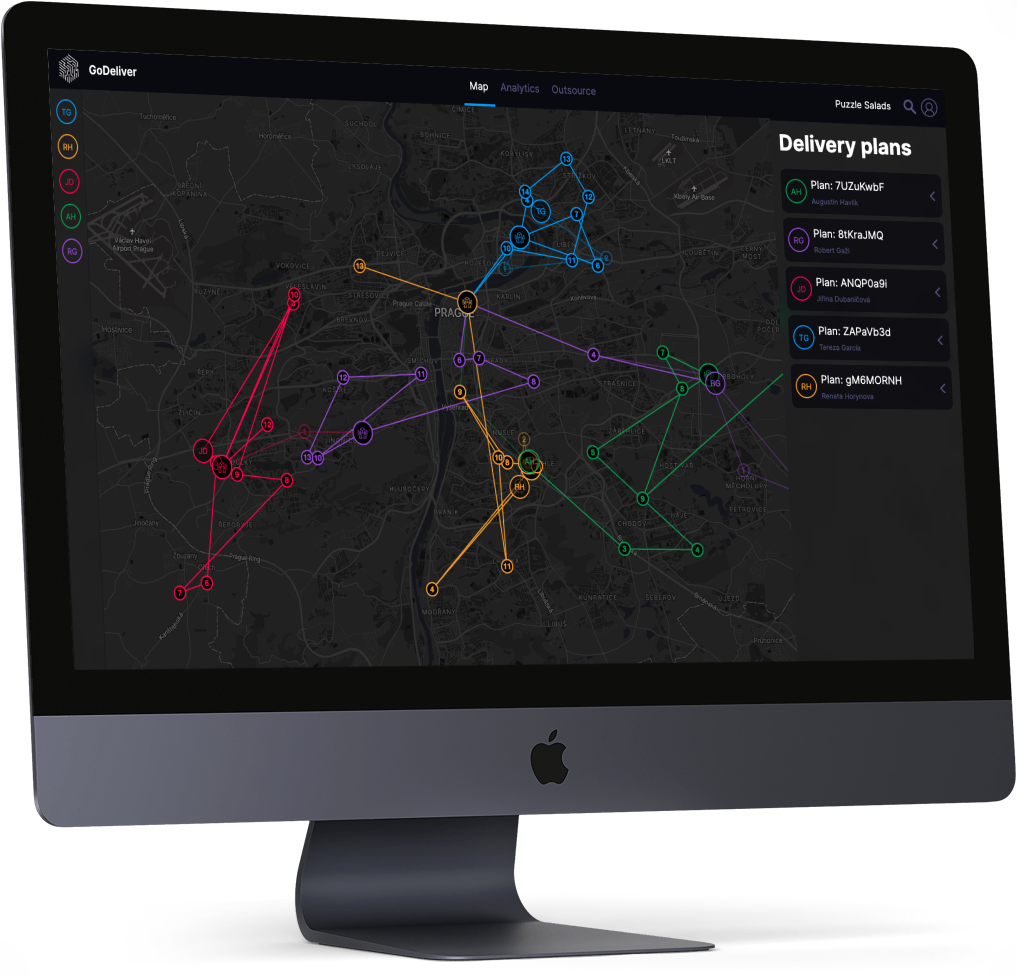
\includegraphics[width=0.5\textwidth]{resources/intro/godeliver-dashboard.png}
        \caption{GoDeliver dashboard visualizing solution for an instance of vehicle routing problem with time windows.}
        \label{fig:godeliver_dashboard}
    \end{figure}
    
    \section{Motivation}
    The paradigm shift in logistics business models towards instant gratification of customers are pushing the planning systems to be flexible and dynamic. The environment is constantly changing and planning systems have to update or entirely replan the instance in a short amount of time but maintaining the best delivery efficiency. Having a powerful planning system results in a dramatic reduction of delivery expanses.
    
    \section{Challenges}
    In the real world, the general VRP problem is not enough to solve the business-related problems. \gls{vrp} has multiple variants adding various constraints such as capacity, demand or time windows for given set of customers. The \gls{vrptw} is main focus of this thesis and we will be looking at some novel approaches how to solve it with \gls{ai}.
    
    \section{Assumptions} 
    We expect that leveraging \gls{ai} or \gls{ml} techniques to solve \gls{vrp} would lead in a drastic reduction of computational time for solving given instance of \gls{vrp}. Moreover, the time complexity would not be exponentially increasing with the problem size. The trade-off lays in the required time to allow \gls{ai} to train and learn how to solve the problem of vehicle routing.
    
    \section{Thesis structure}
    The rest of this thesis is organized as follows:
    \begin{itemize}
        \item Chapter \ref{introduction_vrp} presents a formal introduction to Vehicle Routing Problem.
        \item Chapter \ref{theoretical_background} provides an advanced theoretical background.
        \item Chapter \ref{vrptw-optimization} describes solutions of \gls{vrptw} for optimization heuristics.
        \item Chapter \ref{system} describes how a delivery planning system works.
        \item Chapter \ref{vrptw-ai} describes the proposed method for solving \gls{vrptw} via deep learning.
        \item Chapter \ref{evaluation} evaluates and benchmarks the proposed deep learning model.
    \end{itemize}
\end{introduction}
    \chapter{Introduction}
    The \gls{vrp} is one of the most extensively studied combinatorial problems. It is easy to define but hard to solve. The reason (\gls{vrp}) is attracting many researchers is the fact that finding a near-optimal solution in a reasonable time would have a great impact on many industries, especially in the domain of transportation and logistics. 
    
    The paradigm shift in logistics business models towards instant gratification of customers are pushing the planning systems to be flexible and dynamic. The environment is constantly changing and planning systems have to update its solutions in a short amount of time but maintain the best delivery efficiency.
    
    The problem objective of \gls{vrp} is simply finding the shortest route for multiple vehicles to serve all the given set of customers. The shortest route can be differently interpreted based on your minimalization criteria, e.g, traveled distance, time, or a combination of both. It was first proposed by Dantzig and Ramser \cite{truck-dispatching-problem} in 1959, and since then researchers are coming up with different approaches how to solve the problem. 

    In the real world, the general VRP problem is not enough to solve the business-related problems. \gls{vrp} has multiple variants adding various constraints such as capacity, demand or time windows for given set of customers. The \gls{vrptw} is main focus of this thesis and we will be looking at some novel approaches how to solve it with \gls{ai}.
    
    Solving any kind of variation of \gls{vrp} via \gls{ai} results in instant geneated solution. Solving any kind of variation of \gls{vrp} via \gls{ai} results in instant geneated solution. Solving any kind of variation of \gls{vrp} via \gls{ai} results in instant geneated solution. Solving any kind of variation of \gls{vrp} via \gls{ai} results in instant geneated solution.
    
    \begin{figure}[ht]
        \centering
        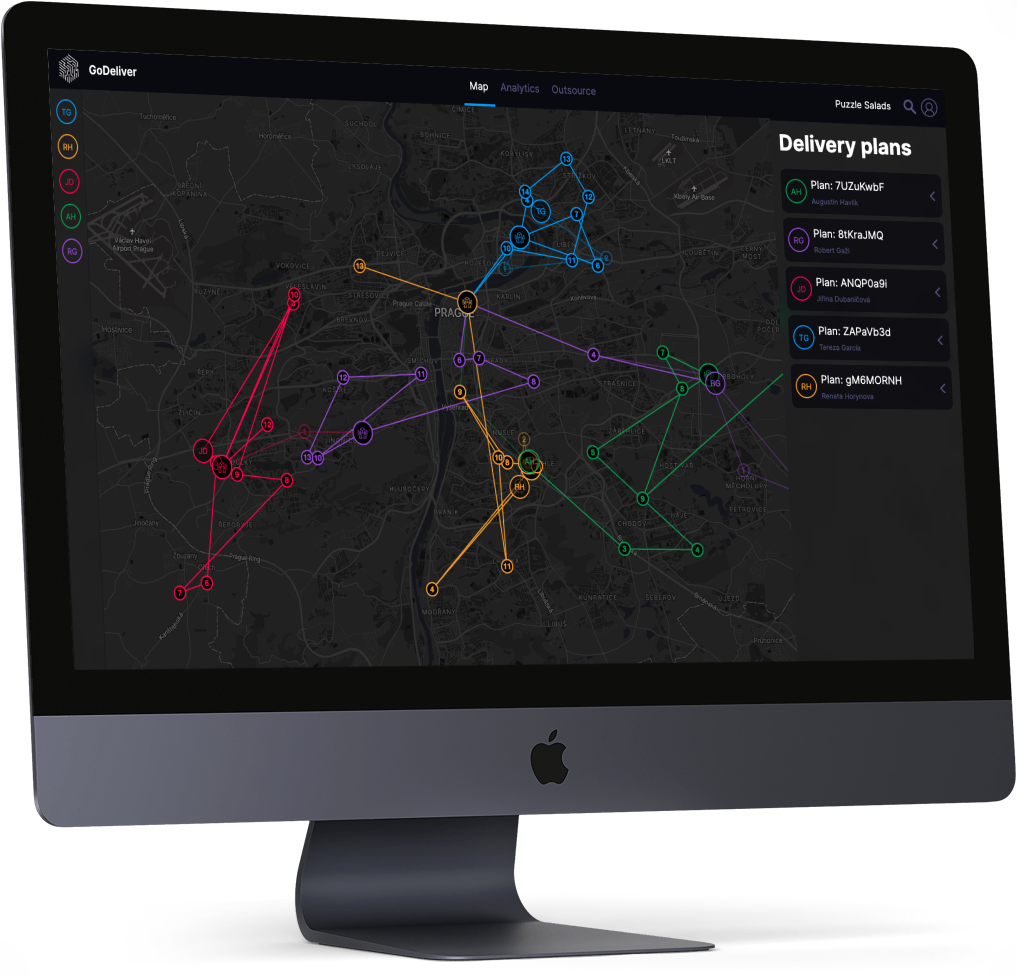
\includegraphics[width=0.75\textwidth]{resources/intro/godeliver-dashboard.png}
        \caption{GoDeliver dashboard illustrating the vehicle routing problem with time windows}
        \label{fig:godeliver_dashboard}
    \end{figure}

\section{Vehicle Routing Problem Definition}
    
    The general \gls{vrp} can be defined as a problem in a complete graph $G=(V,E)$ of finding the optimal permutation $\pi_l = (\pi_0, \cdots, \pi_m)$ of nodes $V$ all starting from a node $v_0$ for given number of paths $k$ which results in minimal traversal cost where $\forall v \in (V \setminus v_0)$ are visited only once. \gls{vrp} is generalization of \gls{tsp} which only has one path.
    
    \begin{figure}[ht]
        \centering
        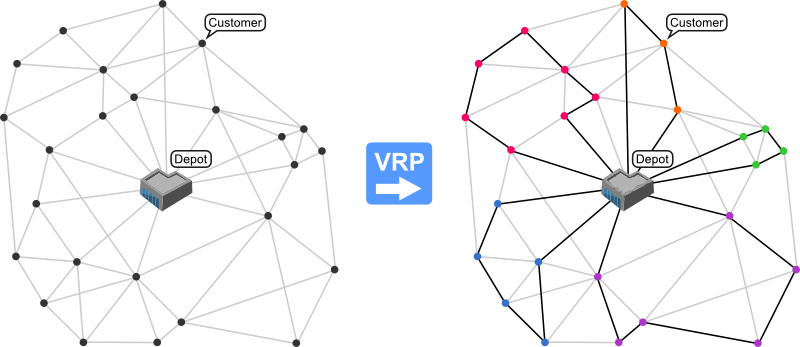
\includegraphics[width=0.75\textwidth]{resources/intro/vrp-graph.png}
        \caption{Intuitive view of \gls{vrp} instance on left and proposed solution for 5 vehicles on the right \cite{vrp-malaga}}
        \label{fig:vrp-graph}
    \end{figure}
    
    Let's introduce our used notation and its real-world interpretation.
    \begin{itemize}
        \item $G=(V,E)$ is a complete undirected graph
        \begin{itemize}
            \item Network of routes
        \end{itemize}
        \item $v_0$ is the initial node
        \begin{itemize}
            \item A depot
        \end{itemize}
        \item $V_1 = (v_1, \cdots, v_n)$ nodes expect the initial node
        \begin{itemize}
            \item Geographically scattered location of customers
        \end{itemize}
        \item $E = \{(v_i, v_j)| v_i, v_j \in V, i \neq j\}$ with associated weight as a cost $c: E \to \mathbb{N}^+$
        \begin{itemize}
            \item A single route between two locations with associated cost, e.g., distance.
        \end{itemize}
        \item $R_i \subset V$ is a path but starts and ends at $v_0$
        \begin{itemize}
            \item Route visit a subset of customers starting and ending at a depot, it can be referred to it as a delivery plan.
        \end{itemize}
        \item $k$ number of paths
        \begin{itemize}
            \item Number of vehicles
        \end{itemize}
        \item $R = R_1, \cdots, R_k$ is a set of paths
        \begin{itemize}
            \item All routes (delivery plans) for a given instance of \gls{vrp}.
        \end{itemize}
        \item $\pi = (\pi_1, \cdots, \pi_k)$ solution for a given instance of \gls{vrp}.
        \begin{itemize}
            \item Customer locations in visiting order for multiple vehicles.
        \end{itemize}
    \end{itemize}
    
    Solution for \gls{vrp} of routes $R_k$ is feasible only if each node $V_1$ is visited once.
    
    The cost of route $R_i$ which we aim to minimize is the sum of its weights (costs). If we operate in Euclidean space, then it is L2 norm of route locations.
    \begin{equation}
        C(R_i) := \sum_{i \in R} d_i \leq Q TODO
    \end{equation}
    
    The cost of \gls{vrp} solution is a sum of route costs.
    \begin{equation}
        C(R) := \sum_{i \in R} d_i \leq Q TODO
    \end{equation}
    
\section{Vehicle Routing Flavors}
Our modern world heavily relies on complex logistics networks to ship your goods from one side of the world to your doorstep. In order to synchronize This takes a multi-modal planning be planned and that is the reason why other flavours and varients of \gls{vrp} has been studied and implemented in real world usecases.

    \begin{figure}[ht]
        \centering
        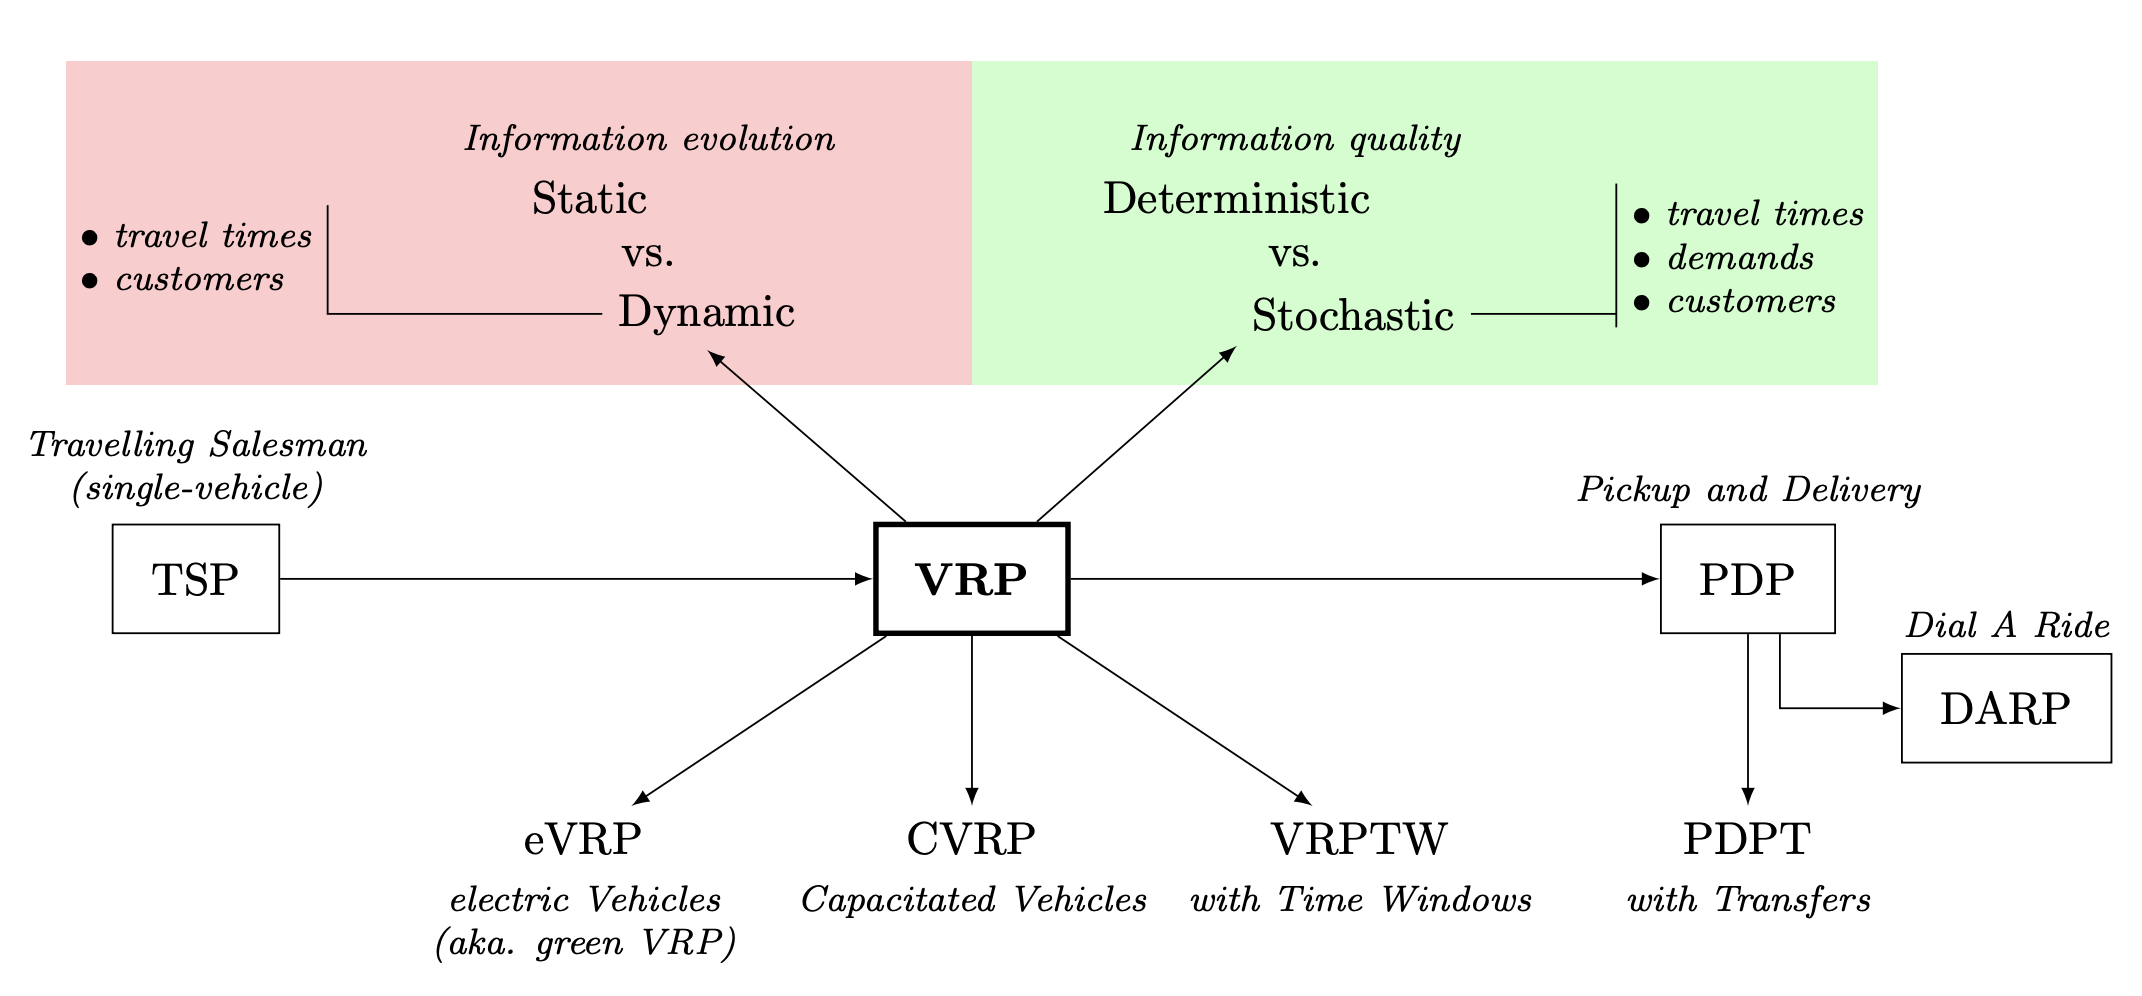
\includegraphics[width=1.0\textwidth]{resources/intro/vrp-flavours.png}
        \caption{Taxonomy of VRPs \cite{bono-stochastic-vrp}}
        \label{fig:vrp-flavours}
    \end{figure}

The sections bellow will be desctibing each flavours of shown in \ref{fig:vrp-flavours}

    \subsection{Capacited Vehicle Routing Problem}
    The \gls{cvrp} extends the regular \gls{cvrp} in introducing a capacity element for each customer. In the literature, it is sometimes referred to as a demand. The customer's demand is $d \in \mathbb{N}^+$ which may represent capacity in the form of weight, size but also in some abstract concepts such as a basket of apples. Additionally, each vehicle has a predefined capacity $Q > 0$.
    
    The \gls{cvrp} extends the solution feasibility formula by the following capacity constrain.
    \begin{equation}
        q(R) := \sum_{i \in R} d_i \leq Q
    \end{equation}
    
    If the vehicle capacity of the fleet stays the same, we are dealing with \gls{cvrp} with homogenous fleet. A fleet with varying capacity for each vehicle is a heterogenous fleet.
    
    \subsection{Vehicle Routing Problem with Time Windows}
    The \gls{vrptw} extends the regular \gls{vrp} by time constraint for each customer. Customers have assigned time window interval $[e_i, l_i]$ where $e_li < l_i$, is the request when a vehicle is supposed to visit the node. The time window can be either implemented as a hard constraint
    
    We consider time windows as a soft constraint, every time window can be violated barring a penalty cost. 
    
    In this thesis, we will be focusing on soft contrains for time windows because the lead to 
    
    Fesability - soft constraint
    
    \subsection{Pick and Deliver}
    TODO
    \subsection{Static Vehicle Routing Problem}
    TODO
    \subsection{Dynamic Vehicle Routing Problem}
    TODO
    \subsection{Deterministics Vehicle Routing Problem}
    TODO
    \subsection{Stochastic Vehicle Routing Problem}
    TODO
    
\section{Real-world Applications}
 Since then, a large part of the OR community has been devoted
to this problem which naturally arises in a large variety of practical applications. This
trend has been reinforced by the explosion of consumer direct delivery in the beginning of
the century. As an example of this explosion, UPS ground delivered around 11.5 million
packages in 19931
, against around 5.5 billion packages in 20192
.

Vehicle routing problems, among the most studied in combinatorial optimization, arise in many practical contexts (freight distribution and collection, transportation, garbage collection, newspaper delivery, etc.). Operations researchers have made significant developments in the algorithms for their solution, and Vehicle Routing: Problems, Methods, and Applications, Second Edition reflects these advances. The text of the new edition is either completely new or significantly revised and provides extensive and complete state-of-the-art coverage of vehicle routing by those who have done most of the innovative research in the area; it emphasizes methodology related to specific classes of vehicle routing problems and, since vehicle routing is used as a benchmark for all new solution techniques, contains a complete overview of current solutions to combinatorial optimization problems. It also includes several chapters on important and emerging applications, such as disaster relief and green vehicle routing. Audience: This book is intended for both researchers and graduate level students in operations research and applied mathematics. Practitioners will find this book particularly useful. Readers need a basic knowledge of the main methods for the solution of combinatorial optimization problems.
    \chapter{Related work}\label{related_work}
    In this chapter, we briefly present relevant work addressing similar problems in \gls{mot} and soft-biometrics field. Given the vastness of the topic, we only limit the review to significant work.

\section{\Glsentrylong{mot}}
     Most state-of-the-art algorithms addressing \gls{mot} follow the tracking-by-detection approach, which heavily relies on the performance of the underlying object detector. However, the trend is now shifting to the end-to-end learning solutions and constructing stronger similarity scores based on appearance, motion, and interaction cues. Although recent \gls{nn} based detectors have outperformed all other methods for object detection \cite{russakovsky2015imagenet, ren2015faster, redmon2016you}, \gls{mot} remains a challenging and popular topic.
   
    \Gls{sort} \cite{bewley2016simple} is the first pragmatic approach where the main focus is to associate objects efficiently for online and real-time applications. They showed that the quality of detections plays a crucial role in tracking performance and according to their experiments, they can improve tracking by almost 20 \%, depending on the detector. Despite using an only simple combination of standard techniques as the Kalman Filter for motion prediction and Hungarian algorithm for the association of the tracks, they were able to achieve comparable performance to other state-of-the-art online trackers. 
    
    By adding a deep association metric to \gls{sort} \cite{wojke2017simple}, it was successfully integrated with the appearance model that improves the tracking performance. The appearance model is based on \gls{cnn} trained on large scale person \gls{reid} dataset. Due to this extension, the algorithm can track objects through longer periods of occlusion, effectively reducing the number of identity switches. The framework of this paper is used for our tracking task. Thus it is more explained in the next chapter. 

    In 2016, revolutionary end-to-end learning approach based on \gls{rnn} \cite{mikolov2010recurrent} has been introduced in a novel \cite{milan2017online}. Their proposed \gls{lstm} \cite{hochreiter1997long} architecture is capable of performing all multi-target tracking tasks including prediction, data association, state update as well as initiation and termination of targets within a unified network structure. One of the main advantages of this approach is that it is completely model-free, i.e., it does not require any prior knowledge about target dynamics, clutter distributions, etc. However, the object detections should be given as input.
    
    It was not the only case of successful use of \gls{rnn}. In the paper \cite{sadeghian2017tracking} published year later, a new approach combining multiple cues such as appearance, movement, and interaction is proposed. These cues are fed into \gls{lstm} \cite{hochreiter1997long} architecture, which learns and remembers the dependencies in a sequence of observation, in contrast to pairwise similarity where only the observations from the current and previous frames are used. Their proposed framework follows end-to-end fashion, and their architecture does not require object detections as input.
    
    Competitive tracking results can be achieved even without sophisticated tracking methods. Tractor \cite{DBLP:journals/corr/abs-1903-05625} accomplishes tracking without following the common tracking-by-detection approach and authors performed no training or optimization on tracking data. Instead, they exploited the bounding box regression of an object detector to perform temporal realignment and to predict the position of an object in the next frame. They also provide a simple extension to this approach, in the form of Siamese \gls{nn} for \gls{reid} and motion analysis model, which achieve state-of-the-art performance on tracking benchmarks. 
    
    Results of recent tracking evaluations show that bounding box tracking performance is saturating \cite{mot16}. Further improvements will only be possible when moving to the pixel level., which is a reason why the authors of recent 2019 work \cite{DBLP:journals/corr/abs-1902-03604} are expanding from \gls{mot} to \gls{mots}. They propose new TrackR-CNN baseline method which jointly addresses detection, tracking, and segmentation with a single convolutional network that extends Mask R-CNN architecture with 3D convolutions to incorporate temporal information, and by an association head which is used to link object identities over time. They also provide evaluation metrics and new dataset with masks for over one thousand distinct objects in ten thousand frames. The main advantage of \gls{mots} is that segmentation based tracking results, are by definition non-overlapping and can thus be compared to ground truth straightforwardly.
    
\section{Soft-biometrics}
    There has not been much written about the general use of biometrics in retail yet. However, some exceptions exist. For example, in \cite{fookes2010semi} authors propose semi-supervised intelligent multi-camera surveillance framework that can perform multiple tasks, including camera management, camera calibration, and multi-view object tracking with \gls{reid} based on appearance soft-biometric traits. The survey \cite{quintana2016improving} from 2016 provides a complete overview of innovative camera approaches that can be applied in the retail environment. The study \cite{de2018comparative} aims at recognizing the age, gender, presence of eyeglasses and beard of passers-by in a retail store. Their solution lies in custom \gls{cnn} architecture that extracts these traits.
    
    Although end-to-end solution targeting solely retail environment have not been proposed yet, there are plenty of works that deal only with certain soft-biometric features.
   
    \subsection{Body traits}
        Frequent body traits \cite{de2018comparative} extracted from an \gls{rgb} camera are height, gait, and color of clothes. The best feature for distinctiveness between individuals proved to be gait, which is the reason why it is often used in forensic analysis. However, there are not many uses for gait in the retail environment. Thus we only focus on others.
        
        \subsubsection{Height estimation}
            There has been a long history in determining an individual's height. One of the essential works in this field is \cite{criminisi2002single}, where authors proved that height estimation is possible without any information about camera parameters, only several scene correspondences with known real-world measurements are sufficient. In their work, they also describe how the affine 3D geometry of a scene can be reconstructed from a single image.
            
            In \cite{viswanath2009simplified} authors describe a simple uncalibrated model of error distribution in height as a function of the location of the object in the image and the estimated camera height. Their approach builds on previous work \cite{criminisi2002single} and improves the accuracy in estimating the height while reducing the burden of reliably computing the ground plane. 
        
            More recent work \cite{momeni2012height} uses a single calibrated camera, more explicitly assuming the knowledge about its pose concerning the world and vanishing point in the reference direction. According to their proposed theorem, by knowing the proportion of camera height concerning the object height, at the object’s position in the image plane, it is possible to estimate the height of the object in the real world. Their presented method gives accurate results in unstructured environments, regardless of the relative distance from the camera.
            
            Authors of \cite{li2015simplified} proposed a framework utilizing the calibrated camera for estimating height in video surveillance. Their primary assumption is that it is possible to obtain a camera's focal length, tilting angle, and height by using non-linear regression model from the observer's head and foot points of people in the scene, instead of estimating the vanishing point and vanishing line. Once these calibration parameters of a camera are obtained, the physical height of a person can be estimated from a pair of head and foot points observed from the image and their proposed formula.

        \subsubsection{Color clothes estimation}
            One of the essential works \cite{yamaguchi2012parsing} in this field comes from 2012, where authors focus on fashion photographs and propose an effective method to produce intricate and accurate parse of a person’s outfit. They also introduced large labeled dataset with available labeling tools. Finally, they designed a prototype application for visual garment search.
            
            DeepFashion \cite{liu2016deepfashion} is another large-scale clothes dataset with extensive annotations introduced in 2016. Authors also introduced a new baseline method, namely FashionNet, which learns clothing features by jointly predicting clothing attributes and landmarks. The estimated landmarks are then employed to pool or gate the learned features. 
            
            The current state-of-the-art is the baseline model built upon Mask R-CNN \cite{he2017mask}, termed Match R-CNN \cite{ge2019deepfashion2}. The authors of this work also proposed new challenging large-scale dataset DeepFashion2. Their presented model offers end-to-end training framework that jointly learns clothes detection, landmark estimation, instance segmentation, and consumer-to-shop retrieval. 

    \subsection{Facial traits}
        If we focus only on the head of individuals, then many algorithms targeting facial biometric \cite{wang2018deep} are regularly introduced. Most of the work from this field comes inevitably from face recognition task, which is natural since this field has a history almost as long as fingerprint recognition. Commonly extracted facial soft-biometrics are gender, ethnicity, age, emotion, pose, glasses, beard, and mustache with a frequent goal to explore their discrimination capabilities among other individuals during in-the-wild scenarios. We will limit this review to only the most important ones that can be used for retail use, namely age, gender, emotion, and pose \cite{balaban2015deep}. Some of these traits are commonly estimated together by using one model.
        
        \subsubsection{Multi-task approaches}
            In paper \cite{yin2018multi}, authors propose multi-task \gls{cnn} for face recognition where identity classification is the main task and pose, illumination, and expression estimations are the side tasks. They also provide analysis of multi-task learning with extensive experiments that demonstrate the effectiveness of the proposed approach.
            
            HyperFace \cite{ranjan2019hyperface} is an algorithm that can simultaneously do face detection, landmarks localization, pose estimation and gender recognition. It uses \gls{cnn} model architecture that fuses intermediate layers of a \gls{cnn} using a separate \gls{cnn} followed by a multi-task learning algorithm that operates on the fused features. It exploits the synergy among the tasks which boosts up their performances. They also proposed two variants with a different focus -- HyperFace-ResNet that achieves high accuracy and Fast-HyperFace that significantly improves the speed of the algorithm. Their experiments show that the proposed models can capture both global and local information in faces and perform significantly better than many competitive algorithms for each of these four tasks.
            
            The authors of the same composition later released improved version \cite{ranjan2017all} that can additionally solve for tasks of smile detection, age estimation, and face recognition. They also extended their approach by training the model on multiple datasets whereas HyperFace was trained only on one. 

        \subsubsection{Age and gender estimation}\label{age_and_gender_estimation_related}
            In most retail cases, we are interested in estimating age at the same time as gender \cite{ranjan2017all, wang2015deeply}, since these traits play a crucial role in targeted advertising. In the case of age, it is very challenging to obtain it by the camera because the apparent age sometimes significantly differ from the real one. Fortunately, particular numbers are not that important, but instead categories such as child, youth, adult, middle-age and elderly. On the other hand with gender, the situation is slightly simpler because there are several other attributes that algorithms can use. We further present only recent proposals from this field that mostly relies on \gls{dl} models. 
            
            The first ever work applying \gls{dl} methods was presented by the authors in \cite{wang2015deeply}. They propose a \gls{cnn}-based framework for age estimation, and instead of using only the feature map obtained at the top layer, they utilize feature maps obtained in different layers for the final estimation. Additionally, they incorporate a manifold learning algorithm in the proposed scheme, and that significantly improves the performance.

            In the same year, work \cite{rothe2015dex} introduced \gls{dex} method that tackles the estimation of apparent age in face images. They proposed \gls{cnn} with VGG-16 architecture pre-trained on ImageNet. They also introduced large-scale face images dataset with available age to pre-train their \gls{cnn}. 

            Recently in 2019, authors of \cite{yang2018ssr} proposed \gls{ssr}, a light-weight \gls{cnn} model with real-time performance that is targeting age and gender estimation. Their work is inspired by DEX, and they address age estimation by performing multi-class classification and then turning classification results into regression by calculating the expected values. Their greatest benefit is the compactness of the model presented. \Glsentryshort{ssr} takes only 0.32 MB of memory, and despite its size, it is approaching the performance of more than 1500× larger state-of-the-art methods.
            
        \subsubsection{Facial expression recognition}
            Facial expression \cite{goodfellow2013challenges} is one of the main clues that can be utilized in retail stores to measure the satisfaction of the consumers. \cite{arriaga2017real} is a very popular paper that proposes a general \gls{cnn} framework with real-time performance. Their model is capable of accomplishing the tasks of face detection, gender classification, and emotion classification simultaneously in one blended step using the proposed architecture. They validate their results on recent datasets, but also by building their robot which succeeded in the competition. Their architecture and pre-trained models are released under an open-source license.

            The framework known as EmoPy \cite{emopy} is a toolkit with multiple implemented \gls{cnn} architectures for emotion recognition. For example, they use time-delayed 3-D \gls{cnn}  that utilizes temporal information as part of its training samples. In other words, instead of using an only single image for prediction, it uses past images from a series for additional context. The idea is to capture the progression of a facial expression leading up to a peak emotion. They also propose hybrid \gls{lstm} \cite{hochreiter1997long} architecture that combines approaches from \gls{cnn} and \gls{rnn} to include temporal context from whole still images, not only from face patches as the former presented. They also introduce a simpler model trained on FER2013 dataset \cite{goodfellow2013challenges} which can make predictions based on a single image. Moreover, in their framework, it is possible to specify only a smaller subset of all seven emotions available, which is undoubtedly more practical in real-world scenarios.
            
            Paper \cite{zeng2018facial} from 2018 has presented a novel approach for facial expression recognition using \gls{dsae} \cite{sun2016sparse}, which can automatically distinguish the expressions with high accuracy. Both the facial geometric and appearance features have been introduced to compose a high-dimensional feature with accurate and comprehensive information of emotions. In the end, the experiment results have demonstrated that the proposed approach outperforms the other three state-of-the-art methods by a large margin.
             
        \subsubsection{Head pose estimation}
            Head pose estimation \cite{wang2018deep} is closely related to other facial analysis problems, and it might be useful in a retail store when there is a requirement for modeling customer attention on specific products or areas. Traditional algorithms work by estimating facial landmarks (key points) from the target face and then solving the 2D to 3D correspondence problem with a mean human head model as a reference. Since it is a very fragile method that relies on landmark detection performance, current state-of-the-art methods focus on detecting the pose without detecting the key points. 
            
            In 2018, an accurate and easy to use head pose estimation \gls{cnn} known as Hopenet \cite{Ruiz_2018_CVPR_Workshops} was introduced. In their work, authors can detect intrinsic Euler angles (yaw, pitch, and roll) directly from image intensities through joint binned pose classification and regression. They showed their network generalization capacity by testing the performance on various external datasets without fine-tuning. 
        
            A novel method is known as FSA-Net \cite{fsanet} also targets head pose estimation. Authors of this work proposed a light-weight non-landmark \gls{cnn} model that even outperforms methods utilizing multi-modality information from depth and \gls{rgb} cameras.
    \chapter{Methodology}\label{methodology}
    This chapter provides an overview of our designed procedures and algorithms. As mentioned in the earlier in the thesis objectives, the goal is to design and implement a framework that tracks people in the video sequence followed by additional information extraction on person-specific features. Before getting into our the tracker design, we present our data acquisition and data pre-processing process. Later then, we propose a people detector and tracker which follows the well-known tracking-by-detection approach and in the end, we present strategies for additional information extraction. 

\section{Image acquisition}
    Image acquisition is the first stage in any vision processing system. The goal of image acquisition is to transform real-world optical data into an array of numbers that can be processed by a computer. The process heavily depends on the camera and lens hardware. 
    
    The main component of the camera is its sensor that converts light into electrical charges, while the lens focuses the light on particular spots of the sensor. Nowadays, the most used technology for the camera sensor is \gls{cmos} due to its low noise and processing speed capabilities. Since the work is done in cooperation with well-equipped \gls{improlab} at \gls{fit} \gls{ctu}, we have a choice of several camera and lens variants available.
    
    Based on assumptions and thesis instructions, we know the scene, and its parameters in advance. To test the designed algorithms of this work, we chose the scene to be the 14th floor of the \gls{fce} \gls{ctu} building near elevators. Based on the scene, we selected the appropriate combination of lens and camera sensitive to the visible spectrum. The \gls{improlab} has most of its cameras from Basler manufacturer. Thus we decided to utilize Basler ace acA1920-50gc \cite{baslercamera}, the \gls{gige} camera with the Sony IMX174 \gls{cmos} sensor that delivers 50 \gls{fps} at 2.3 \gls{mp} resolution. Due to the spatial properties of the scene, we chose Basler 8mm lens C125-0818-5M F1.8 \cite{baslerlens} that proved to be the best option in this case.
   
    \begin{figure}[h]
        \centering
        \subfloat[]{{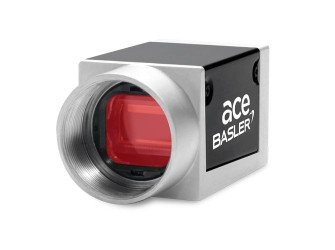
\includegraphics[width=0.35\textwidth]{resources/basler_camera.jpg} }}
        \qquad
        \subfloat[]{{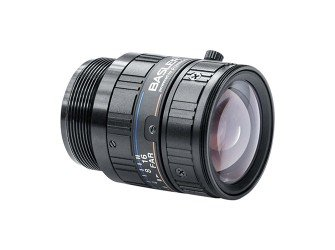
\includegraphics[width=0.35\textwidth]{resources/basler_lens.jpg} }}
        \caption{Selected camera equipment for our task. a) Camera Basler ace acA1920-50gc. b) Lens Basler 8mm  C125-0818-5M F1.8. Source: \cite{baslercamera, baslerlens}}.
        \label{fig:camera_equipment}
    \end{figure}
    
    The image stream from Basler's camera equipment can be obtained in several ways. The most convenient but limiting approach is to use Basler pylon Camera Software Suite, which is a software package comprised of an easy-to-use \gls{sdk}, drivers and tools that can be used to operate any Basler camera using the user interface on multiple platforms such as Windows, Linux, and Mac. However, this option does not allow integration with custom software. Another option is to use Basler's pypylon \cite{baslerpypylon} which is the new open source wrapper interface for the Basler pylon Camera Software Suite that allows direct camera access through Python code.
    
    Due to the nature of the work, the data can be in an offline form. Thus we decided to use the first method with the Basler pylon framework because it is more convenient than the pypylon wrapper.
    
    We record the video sequence at the highest possible resolution, i.e., 1920x1080 and at 25 \gls{fps}. Each frame is saved in a jpg format to avoid an overhead that would be caused by decoding the video formats. The camera shutter speed is set manually so that people in the scene are not motion blurred and the aperture is set to the sweet-spot of the lens, which in our case is f/4.0, to achieve maximum image quality. Since these parameters would make the image too dark, it is necessary to increase the sensor gain value. In this case, we decided to set sensitivity value to automatic, which means that it is always calculated so that the scene is exposed correctly.  We set the white balance to a fixed value determined by automatic detection to avoid drastic color changes during shooting. We provide an example of the scene in Fig. \ref{fig:scene_example}.

    \begin{figure}[ht]
        \centering
        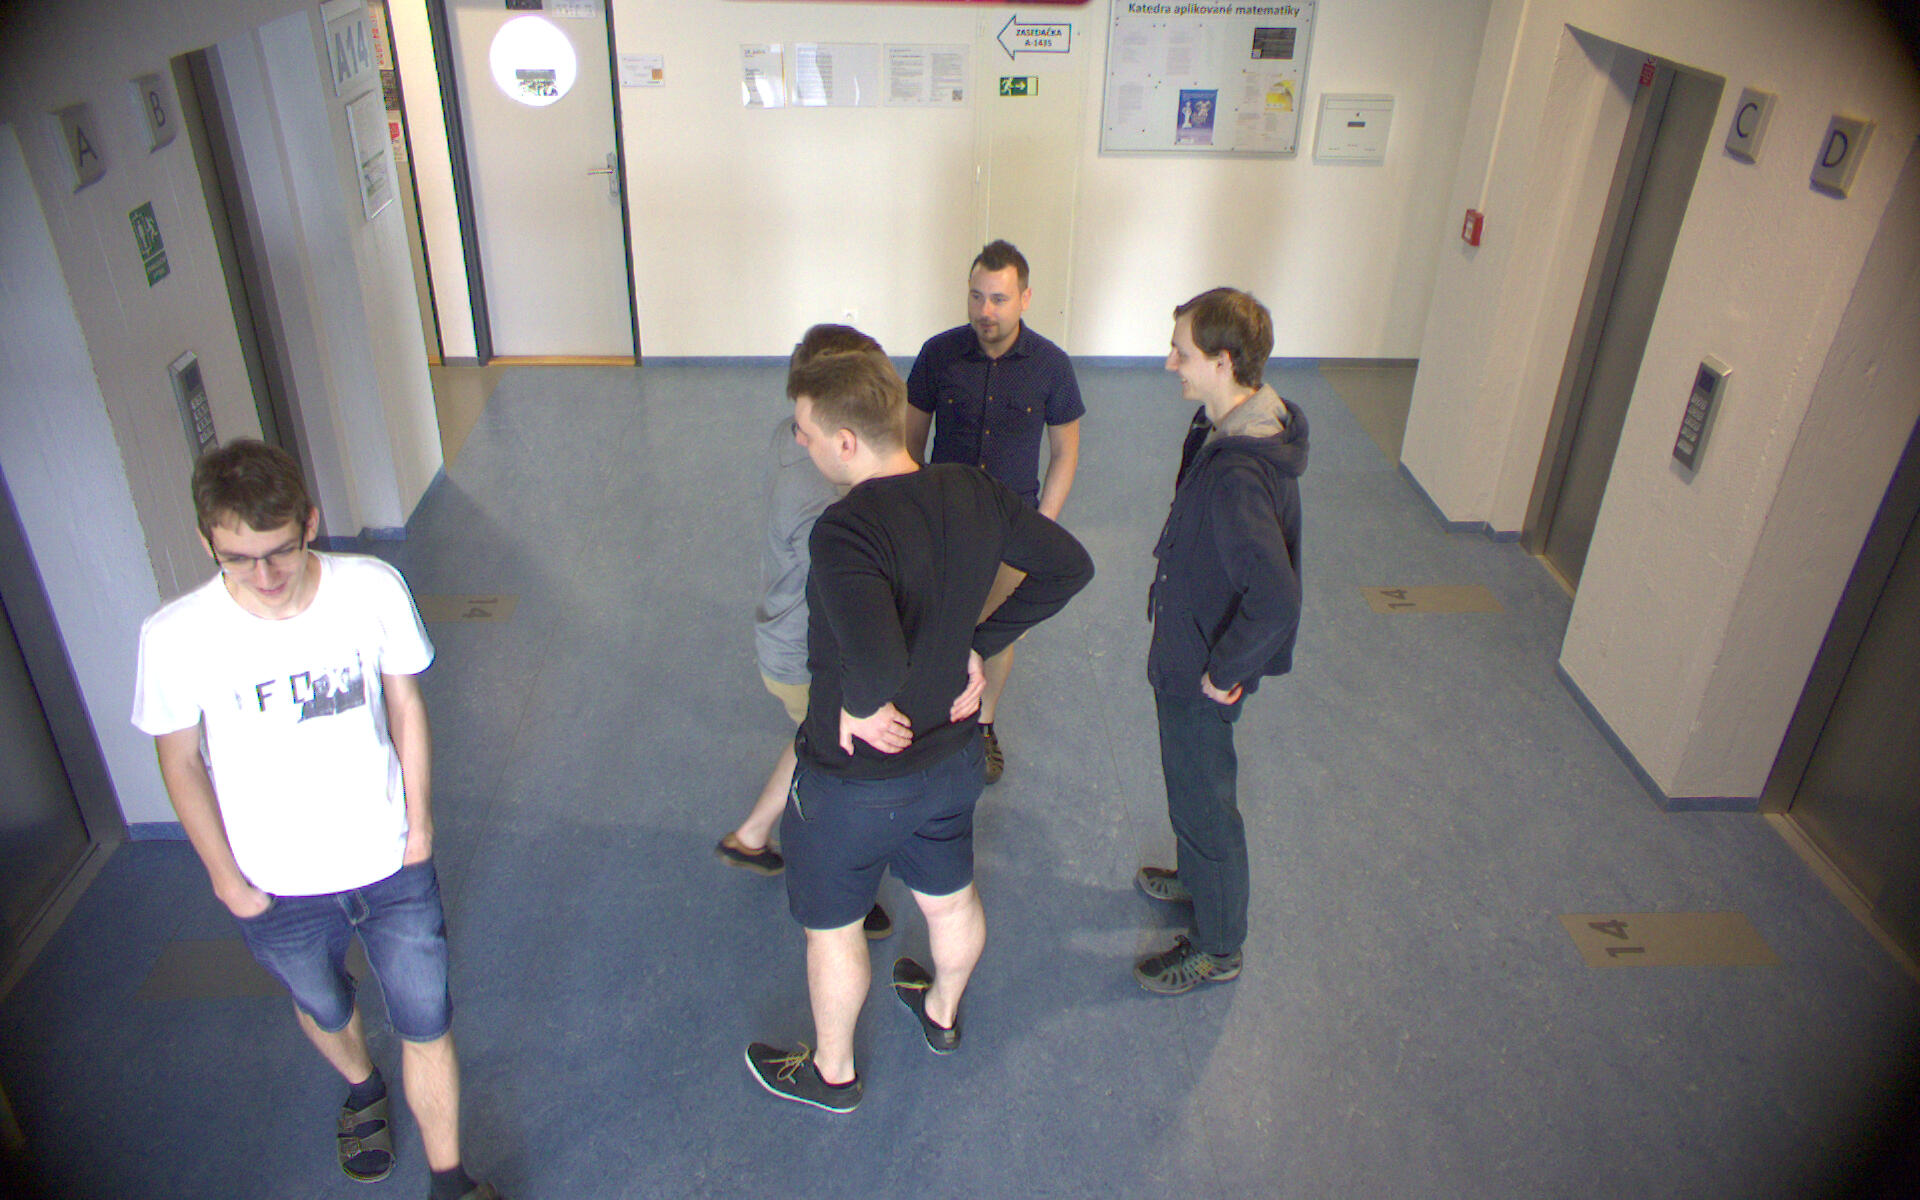
\includegraphics[width=0.75\textwidth]{resources/scene_example.png}
        \caption{Example of the acquired image and the scene layout. We can see that despite being a quality lens, it contains distortion and vignetting.}
        \label{fig:scene_example}
    \end{figure}
        

\section{Image pre-processing}
    After the images are obtained, various pre-processing methods can be applied to improve the accuracy of feature extraction and classification methods. However, in our case, we assume that all images are acquired in satisfactory quality and with proper exposure, shutter speed, and white balance settings. The only pre-processing we do is removing lens distortion by using a camera calibration method as described in \ref{camera_calibration}.

\section{Detection and tracking components}\label{detection_and_tracking_components}
    In this section, we present our design decisions for two core components of our framework -- the detector and the tracker. In contrast to batch based approaches, we primarily target online tracking where only information from the previous and current frame is available. We also try to maintain both components as much as efficient as possible for further extension to real-time applications.

    The \gls{mot} can be viewed as a data association problem, where the goal is to associate hypotheses obtained from the object detector across frames in a video sequence. One way to solve this problem is to compare and match specific features such as the appearance and motion of objects in the scene. 
    
    The methods employed in the tracker are inspired by work \cite{2016arXiv160502688short}, that performs Kalman filtering \cite{kalman1960new} in image space and frame-by-frame data association using the Hungarian method \cite{jonker1987shortest} with an association metric that measures bounding box overlap, and by \cite{wojke2017simple} that improves the previous approach by adding deep association metric.

    \subsection{People detection}
        The beginning of the tracking process is an object detection step. In this work, we use various detector models based on \gls{yolo} and \gls{faster r-cnn} with ResNet50 backbone. The result of forwarding the frame through \gls{cnn} architecture is in the form of hypotheses that contains bounding box coordinates, object class, and detection confidence. Except for input image resizing to be compatible with the \gls{cnn}, we do not perform any other pre-processing in this phase.
        
        Object detectors are usually trained on multiple object classes, but as we are only interested in people, we filter out all other classes from the output hypotheses. We also filter out low-confidence ones. The confidence threshold is variably configured according to the object detector used. \Gls{faster r-cnn} produces a lot of false positives. Thus we take into account only hypotheses with confidence greater than 90 \%. In \gls{yolo}, the threshold value of 70~\% has been experimentally verified to work well. We employ both network architectures with their default parameters trained on the COCO dataset \cite{lin2014microsoft}. 
        A common problem of object detectors is that they often generate more overlapping hypotheses than the ground-truth objects (false positives). To handle the removal of overlapping bounding boxes we use additional \gls{nms} step \cite{rosebrocknms} for bounding box post-processing.
        
        \begin{figure}[ht]
            \centering
            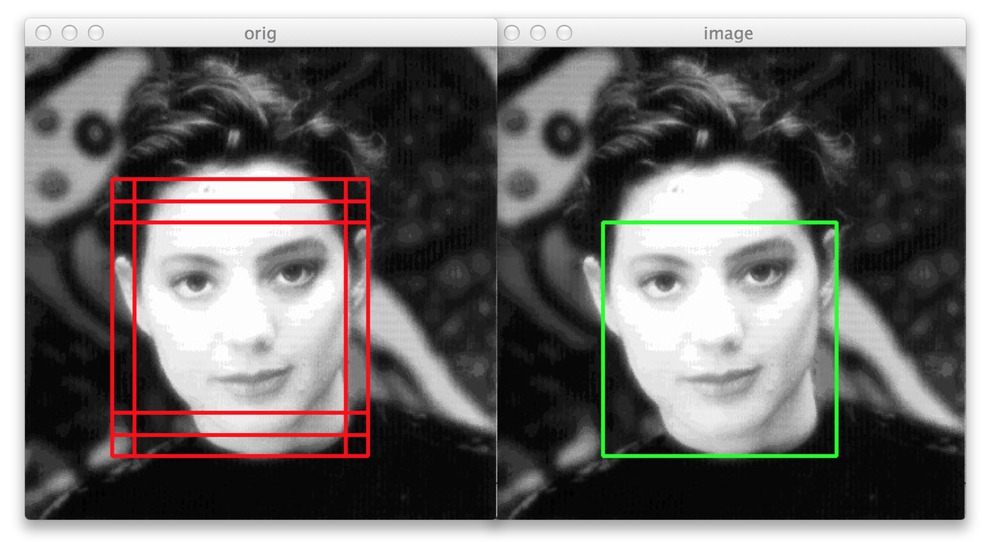
\includegraphics[width=0.75\textwidth]{resources/non_maximum_surpression.png}
            \caption{Six bounding boxes are detected around the face, but by applying non-maximum suppression, it is possible to remove the redundant ones. Source: \cite{rosebrocknms}.}
            \label{fig:non_maximum_surpression}
        \end{figure}
        
    \subsection{Track handling}
        To maintain object identities and propagate object states into the future, we need to maintain historical information in the memory about previous detections. To achieve this goal, we define track object class, and in each frame, we associate current detections with existing track objects (tracks). While the detected hypothesis is only represented by an object class, bounding box and confidence, a track contains multiple attributes such as identity, status, time since the last update, age in frame units, bounding box, state, and class-specific information.
        
        When a person enters or leaves the scene, unique identity needs to be created or removed accordingly. For initiating a new track, we take detections that were not successfully associated in the matching phase of the current frame (unmatched detections). These fresh tracks are then set to tentative during their first $t_c$ frames. Tracks that are not successfully associated during the $t_c$ frames are removed from the scene, which helps to accumulate enough evidence to prevent tracking of false targets. Each track also has a variable that determines the number of frames of the last successful association. Tracks are terminated if they are not associated within $t_m$ frames or their state predictions are outside of the frame. Based on our experiments we have selected a value $t_c = 7$ for track confirmation and $t_m = 50$ for track termination. Due to camera settings, the termination based on our value of $t_m$ means that the appropriate detection was not found for two seconds. 
        
    \subsection{State estimation}
        The state representation helps to propagate a track's identity into the next frames. The inter-frame displacements of each track are approximated with a linear constant velocity model which is independent of other objects. Our design of the track's state is represented as a 10-dimensional vector:
        
        \begin{equation}\label{state_vector}
            x = \left(cx, cy, ty, h, r, \dot{cx}, \dot{cy}, \dot{ty}, \dot{h}, \dot{r} \right), 
        \end{equation}
        
        where $cx$, $cy$ represent center pixel location of the bounding box, $ty$ represent the top center location of the bounding box, $h$ is pixel height, and $r$ is the aspect ratio of the bounding box. Each of these parameters has its respective velocities in image coordinates. 
        
        To predict and estimate the accurate value of track states, we use standard Kalman filter \cite{kalman1960new}. It is a recursive algorithm with a real-time performance that is commonly used to extract the useful signal from noisy measurements. In this case, it can be used to refine the bounding box position. 
        
        The whole filtering process consists of two main steps -- prediction and correction. In the prediction phase, the filter produces predictions of the current state variables, along with their uncertainties. Furthermore, once the output of the next measurement is known, it is used in a correction step to update state variables with a weighted average. The weights are greater for values with higher certainty.
  
        The Kalman filter assumes that the real state at time $k$ can be obtained from state $k - 1$ by the following prediction equation: 
        
        \begin{equation}
            x_k = F_k x_{k-1} + B_k u_k + w_k,
        \end{equation}
        
        where $F_k$ is the  state-transition model, $B_k$ is the control-input model applied to the control vector $u_k$, $w_k$ is the process noise, assumed to be drawn from 
        $w_k \sim {\mathcal {N}} (0,Q_k)$, and $Q_k$ is covariance matrix with appropriate dimensions.
        
        Measurements $z_k$ at time $k$ then can be obtained as follows:
        
        \begin{equation}
           z_{k} = H_{k} x_{k} + v_{k},
        \end{equation}
        
        where $H_k$ is the observation model which maps the true state space into the observed space, $v_k$ is the observation noise, assumed to be drawn from 
        $v_k \sim {\mathcal {N}} (0,R_k)$, and $R_k$ is covariance matrix with appropriate dimensions. All filter parameters are supposed to be correctly user-defined. Otherwise, the filter will not have the required properties.

        In our design, we do not assume the variability of matrices $F_k, Q_k, H_k, R_k$ in time and we can drop $B_k$ since we do not have any control input. $F$ is then designed according to state vector (defined in \ref{state_vector}) and constant velocity model as follows:
        \begin{equation}
            F = 
            \begin{pmatrix}
                1 & 0 & 0 & 0 & 0 & dt & 0 & 0 & 0 & 0 \\
                0 & 1 & 0 & 0 & 0 & 0 & dt & 0 & 0 & 0 \\
                0 & 0 & 1 & 0 & 0 & 0 & 0 & dt & 0 & 0 \\
                0 & 0 & 0 & 1 & 0 & 0 & 0 & 0 & dt & 0 \\
                0 & 0 & 0 & 0 & 1 & 0 & 0 & 0 & 0 & dt \\
                0 & 0 & 0 & 0 & 0 & 1 & 0 & 0 & 0 & 0 \\
                0 & 0 & 0 & 0 & 0 & 0 & 1 & 0 & 0 & 0 \\
                0 & 0 & 0 & 0 & 0 & 0 & 0 & 1 & 0 & 0 \\
                0 & 0 & 0 & 0 & 0 & 0 & 0 & 0 & 1 & 0 \\
                0 & 0 & 0 & 0 & 0 & 0 & 0 & 0 & 0 & 1 \\
            \end{pmatrix},
        \end{equation}
        where $dt$ is chosen to be 1. Matrix $H$ for obtaining measurements is given by:
       \begin{equation}
            H = 
            \begin{pmatrix}
                1 & 0 & 0 & 0 & 0 & 0 & 0 & 0 & 0 & 0 \\
                0 & 1 & 0 & 0 & 0 & 0 & 0 & 0 & 0 & 0 \\
                0 & 0 & 1 & 0 & 0 & 0 & 0 & 0 & 0 & 0 \\
                0 & 0 & 0 & 1 & 0 & 0 & 0 & 0 & 0 & 0 \\
                0 & 0 & 0 & 0 & 1 & 0 & 0 & 0 & 0 & 0 \\
            \end{pmatrix}.
        \end{equation}
        The noise matrices are heavily dependant on the captured scene, but generally speaking, we set significantly higher variance values in for measurement noise matrix $R$ then process noise matrix $Q$. This is because an object detector produces sparse detections with noisy bounding box predictions.

        To sum it up, each track has its state as defined in \ref{state_vector}. When detection is associated with a track, the bounding box coordinates are used as a measurement to update the internal state of the filter. Velocity components are then solved optimally via the filter's transition matrix. If detection is not associated with a track, its state is predicted using a linear model (skipping the correction step). 
        
        More details on the filter assumptions, properties and calculations can be found in its original proposal \cite{kalman1960new}.

    \subsection{Appearance features}\label{appearance_features}
        Using only state estimation in the matching phase would result in a high number of identity switches due to occlusion effects and non-linearity in people's behavior. Therefore, appearance descriptors are often extracted to make hypothesis-to-track matching more robust. At the beginning of this work, we tried to use color histograms of bounding box patches as appearance descriptor. Patches were then converted to \gls{hsv} color space to make them comparable by Bhattacharyya distance \cite{choi2003feature} with hue and value channel as input. However, object histograms are greatly affected by their background. Thus this solution was not robust, and we decided not to continue this path.
        
        Instead, we utilized a \gls{cnn} model from \cite{wojke2017simple} that has been trained to discriminate pedestrians on a large-scale dataset. The input of the model is a bounding box patch of a person and based on that it outputs 128-dimensional vector comparable with cosine distance metric. Through the integration of this feature descriptor, it is possible to recover track's identities even in long-term occlusions.

    \subsection{Data association}
        To create associations between existing tracks and newly arrived detections it is convenient to solve the assignment problem using the Hungarian algorithm \cite{jonker1987shortest}. The values of cost matrix are calculated through a combination of two appropriate metrics -- state and appearance. 
        
        \subsubsection{State metric}\label{state_metric}
            The cost of the state between track and detection is designed in two variants. The first approach is following the design of \cite{wojke2017simple} that uses squared Mahalanobis distance between track states and detections. Since it includes a covariance matrix, it takes into account estimation uncertainty and is defined as follows:
            \begin{equation}
                d_m(i,j) = \left(d_j - y_i\right)^T S_i^{-1} \left(d_j - y_i\right), 
            \end{equation}
            where $y_i$ is $i$-th track state without velocities, $S_i$ is according to state covariance matrix, and $i_j$ is the $j$-th bounding box in an appropriate format. The Mahalanobis distance measures how many standard deviations is the detection away from the mean track location. Its value can then be compared and gated against the proper threshold from a cumulative $\chi^2$ distribution. 
            
            However, it has proven to be inappropriate for our use based on several experiments. The results often diverged, mostly because we try to approximate non-linear person behavior with a linear filter. Therefore, we decided to use a simpler metric with fewer input parameters. More specifically, the Euclidean distance:  
            \begin{equation}\label{eclidean_distance}
                d_e(i,j) = \sqrt{\left(cx_i - cx_j\right)^2 + \left(ty_i - ty_j\right)^2}, 
            \end{equation}
            where $cx_k$ is the $x$ value of center point and $ty_k$ is the $y$ value of top center point of the $k$-th bounding box. Furthermore, we enhance \ref{eclidean_distance} formula so that the output values are in the same order as the outputs of the appearance distance metric:
            \begin{equation}
                d_{el}(i,j) = log_{\alpha}\left(\sqrt{\left(cx_i - cx_j\right)^2 + \left(ty_i - ty_j\right)^2}\right) - 1.
            \end{equation}
            To suppress possible negative values that would not make sense for distance metrics, we take $ \max \left(d_{el}(i,j), 0 \right)$. Our idea behind this formula is that we want to tolerate small spatial displacements caused by the detector in consecutive frames. 
            
            The tolerance amount depends on the base of the logarithm $\alpha \in \mathbb{N}$, which is a hyperparameter that needs to be manually determined based on the task being solved. The influence of $\alpha$ can be best explained by an example. If $d_e(i,j) \leq \alpha$ then $d_{el}(i,j) = 0$, which briefly means that this metric does not penalize bounding boxes that are maximally $\alpha$ pixels distant. 
            The logarithm function then helps to squash the values to lower order. For our type of captured scene, $\alpha = 80$ pixels proved to be working well. 
            
            For the sake of clarity, we provide plot in Fig. \ref{fig:state_formula_plot} of this distance function with $\alpha = 80$.
            
            \begin{figure}[ht]
                \centering
                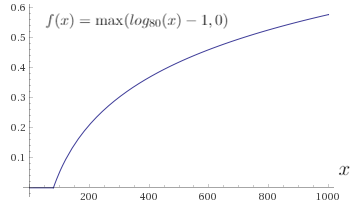
\includegraphics[width=0.55\textwidth]{resources/state_formula_plot.png}
                \caption{Example plot of the distance metric values used for track-to-detection spatial displacement cost.}
                \label{fig:state_formula_plot}
            \end{figure}
            
        \subsubsection{Appearance metric}\label{appearance_metric}
            The appearance metric is used to describe how much are the individuals visually similar, thus helps in distinguishing them. For each detected bounding box patch we calculate its appearance feature vector $r_i$ with $||r_i|| = 1$ by a forward pass of the \gls{cnn} referred in \ref{appearance_features}. Moreover, for each registered track $j$, we keep a gallery $R_j = \left\{ r_j^{(t)}\right\}_{t=1}^{L_j} $ of the last $L_j = 100$ associated appearance features. Then, the appearance distance between the $i$-th detection and the $j$-th track is defined as:
            
            \begin{equation}
                d_{c}(i,j) = \min \left\{ 1 - r_i^T r_j^{(t)} \mid  r_j^{(t)} \in R_j \right\}.
            \end{equation}
            
            The outcome of $d_c(i,j)$ is neatly bounded in $[0,1]$, where $0$ means most similar objects. This time, we introduce a threshold $t_c$ to control if an association is possible. Thus any track and detection pair with $d_c(i,j) > t_c$ is so different that it cannot be associated. For our particular scene, $t_c = 0.15$ has proved to be working well.

        \subsubsection{Matching}
           Building the associations happens in cascade fashion which is taken over from the \cite{wojke2017simple}. The cost value is based on actual state and appearance and is calculated for each possible track and detection pair. We find the best associations by running the Hungarian algorithm \cite{jonker1987shortest} that solves the min cost assignment problem. Then, we verify if the association is possible based on the appearance threshold $t_c$. If yes, we update registered tracks with associated detections. For the rest of unmatched detections, we create new tentative tracks. In Fig. \ref{fig:framework_diagram} we also provide a simplified diagram of one pass through of the algorithm cycle.
           
           \begin{figure}[ht]
                \centering
                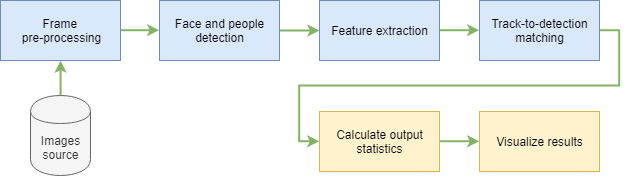
\includegraphics[width=0.75\textwidth]{resources/framework_diagram.png}
                \caption{Simplified diagram of single framework pass through. Yellow-marked boxes are optional components used for evaluation.}
                \label{fig:framework_diagram}
            \end{figure}
            
\section{Soft-biometrics extraction}
    Besides the goal of building the people detector and tracker, we also address additional information extraction related to people class -- soft-biometrics. The aim is to focus on information that can be utilized in the retail environment. Therefore we have focused on methods for estimating age, gender, emotion, height, and ground plane trajectory. Because extraction all of these features in each frame would be computationally intensive, we design our framework to be fully modular in the sense that any of the feature extractors can be turned on or off at any time.
    
    \section{Facial features}
        Before extracting any facial features, robust face detector needs to be utilized to locate faces in the image. Due to the fact the era of traditional methods such as Haar cascades \cite{viola2001rapid} is over, we decided to choose suitable face detector only from \gls{cnn}-based architectures. In particular, we designed an interface for three different \gls{cnn}-based face detectors that offer different trade-offs between speed and accuracy performance. 

        \begin{itemize}
            \item \textbf{faced} \cite{faced} is first of them achieving near real-time performance on \glsentryshort{cpu}. It uses an ensemble of two \gls{cnn}s where first is based on \gls{yolo} architecture. It takes the input image and outputs a grid where each cell contains a prediction of bounding boxes and the probability of one face. Furthermore, these outputs are fine-tuned by another custom \gls{cnn} architecture that is trained to refine bounding box coordinates. Our utilized model is pre-trained on WIDER FACE \cite{yang2016wider} dataset. 
            \item \textbf{Tensorflow Mobilenet SSD} \cite{itzcovichtfdetector} is a popular open-source face detector framework. It is based on a more robust \gls{ssd} \cite{liu2016ssd} architecture than the faced framework, thus it provides better accuracy. We utilize a pre-trained model on WIDER FACE \cite{yang2016wider} dataset that can have a real-time performance on GPU and takes only about 400 MB of \gls{gpu} memory.
            \item \textbf{MTCNN} architecture \cite{7553523} and its implementation \cite{centenomtcnn} is the last utilized face detector that achieves superior accuracy over the state-of-the-art techniques on the public datasets. It leverages a cascaded architecture with three stages of designed \gls{cnn}s to predict face and landmark location in a coarse-to-fine manner. In addition to face detection, it also performs a face alignment. The proposed architecture is a heavy, but it achieves near real-time performance on modern \gls{gpu}s. We use this architecture to compare accuracy performance with weaker face detectors.
        \end{itemize}
        
        Gathered face regions from the face detector need to be paired with people detections. This problem is solved based on the assumption that the face is in the upper middle part of the person bounding box. Face regions with confidence less than 90 \% or without associated person detection are not preserved. No additional post-processing of face regions is done in this step. With the face regions paired to people, we can finally estimate a few types of soft-biometrics.
        
        \subsection{Age and gender estimation}\label{age_gender_estimation}
            As already mentioned in \ref{age_and_gender_estimation_related}, age is most commonly estimated at the same time with gender. In this work, we built an interface for two existing \gls{cnn} models -- Keras Age and Gender \cite{kerasagender} based on \gls{dex} architecture and \gls{ssr} \cite{yang2018ssr}. However, in our specific task, the \glsentryshort{ssr} architecture with the pre-trained model provided not only more accurate predictions but better speed performance. Thus we consider only the \glsentryshort{ssr} in the final design. 
            
            Before feeding the face image patch into \gls{cnn}, we first extend the detected face region by margin $m$ as follows:
            \begin{align}
                x_{tl\textunderscore new} = \max(x_{tl\textunderscore old} - m \cdot fa_w, 0) \\
                y_{tl\textunderscore new} = \max(y_{tl\textunderscore old} - m \cdot fa_h, 0) \\
                x_{br\textunderscore new} = \max(x_{br\textunderscore old} + m \cdot fa_w, fr_w) \\
                y_{br\textunderscore new} = \max(y_{br\textunderscore old} + m \cdot fa_h, fr_h),
            \end{align}
            where $x_{tl\textunderscore new}, y_{tl\textunderscore new}$ and $x_{br\textunderscore new}, y_{br\textunderscore new}$ are new top left and bottom right coordinates of bounding box, respectively, $x_{tl\textunderscore old}, y_{tl\textunderscore old}, x_{br\textunderscore old}, y_{br\textunderscore old}$ are their corresponding original coordinates, $fa_w$ and  $fa_h$ is according width and height of face region,  $fr_w$ and $fr_h$ is according width and height of frame.
            
            If the margin $m$ is too small, then the face is not cropped entirely, and if the offsets are too big, then too much space around the face is included. Both cases affect the prediction accuracy, thus it is necessary to choose a suitable margin for a particular scene. In our case, the value margin value of $m=0.5$ worked well.
            
            Furthermore, face patches are also normalized by min-max normalization from 0 to 255 to eliminate the illumination variance:
            \begin{equation}
                    x_{norm} = \frac{( x - \min(region) ) \cdot (newmax - newmin)}{\max(region) - \min(region)} + newmin,
            \end{equation}
            where $x$ is the input pixel value, $newmin=0$, $newmax=255$, and $\min(region)$ and $\max(region)$ takes accordingly minimum or maximum value of the face region. 
            
           The output of the age classifier is a continuous value which is not further post-processed. Output values from the gender model are $x \in [0,1]$ where $x > 0.5$ means female and otherwise male. The more the value of $x$ is at the edge of the interval, the more certain the prediction is. Also, no further post-processing is needed for gender values.

        \subsection{Facial expression recognition}
            In the same spirit as the previous models, we tried to utilize at least two different architectures to estimate emotions which can be further compared. First of them is \cite{arriaga2017real} inspired by \cite{rothe2015dex} \gls{cnn} architecture, which introduces the open-source framework that can recognize seven types of face emotions -- angry, disgust, fear, happy, sad, surprise, neutral. Their model can operate in real-time, and they provide pre-trained weights on FER2013 dataset \cite{goodfellow2013challenges}. 

            Other architecture employed, known as EmoPy \cite{emopy}, is a toolkit with various \gls{cnn} architectures implemented. However, the most popular model is Fermodel which is trained to predict the same facial categories as the previously mentioned model. We decided to utilize EmoPy for the task of estimating emotions because their framework can operate with a smaller subset of all seven emotions, which is undoubtedly more practical in real-world scenarios. Furthermore, they provide more complex models that provide an output based on temporal information of past frames. The provided model can operate in real-time and is also pre-trained on FER2013 dataset \cite{goodfellow2013challenges}.
            
            For the input of EmoPy, we similarly pre-process the input face region as in \ref{age_gender_estimation}. We expand the face region by margin $m$, but we also convert the image to grayscale. This time, we do not normalize the input image, because the model was not trained in this manner. The output of the model is facial categories with their associated probabilities. We choose the most likely one and ignore the rest.
        
    \section{Spatial information}
        In addition to visual information such as facial features, we can extract additional information which relates to the spatial features of the space captured. However, these methods usually need some knowledge of the scene captured, so they cannot be applied in general. However, in our assumptions, we expected the full knowledge of the scene, thus we are not limited, and we can apply a wide range of available methods.
        
        \subsection{Trajectory}
            One of the most intuitive ways to get some spatial information in the scene is to focus on the movement in space itself. More specifically, extraction of individual's trajectories. The best way to analyze motion in space and to work with trajectories is in the top-down (or bird's eye) view. However, in most real cases of tracking people, we are unable to place the camera to achieve this kind of perspective. This placement would also prevent the possibility of obtaining further facial descriptors. Fortunately, we can transform some parts of the original image to resemble similar to a top-down view. 
            
            Formally, we can utilize 2-D projective transformation between real-world and image ground plane with its main component known as homography matrix. Since the perspective problem is considered as one of the most difficult and precise topics in \gls{cv} that goes beyond the possibilities of this work, we recommend one of the most popular books \cite{hartley2003multiple} in this field, where a detailed explanation can be found. However, if we resort to a brief explanation, then the homography matrix $H$ relates the transformation between two planes (up to a non-zero scale factor $s$) as follows:
            \begin{equation}
                s 
                \begin{pmatrix}
                    x' \\ y' \\ 1 \\
                \end{pmatrix}\
                = H
                \begin{pmatrix}
                    x \\
                    y \\
                    1 \\
                \end{pmatrix}
                =
                \begin{pmatrix}
                    h_{1,1} & h_{1,2} & h_{1,3} \\ h_{2,1} & h_{2,2} & h_{2,3} \\ h_{3,1} & h_{3,2} & h_{3,3} \\
                \end{pmatrix}
                \begin{pmatrix}
                    x \\ y \\ 1 \\
                \end{pmatrix}.
            \end{equation}
            $H$ has eight degrees of freedom, which means there are eight unknowns that need to be solved for, and it is generally normalized with $h_{3,3} = 1$ or $h_{1,1}^2 + h_{1,2}^2 + h_{1,3}^2 + h_{2,1}^2 + h_{2,2}^2 + h_{2,3}^2 + h_{3,1}^2 + h_{3,2}^2 + h_{3,3}^2 = 1$.

            Typically, an estimate of the matrix $H$ is done by finding point correspondences between the target planes. One point correspondence gives two linearly independent equations, and four correspondences are needed for a minimal solution. If more than four correspondences are known, then a more accurate solution can found according to the predefined cost function. Finally, the matrix $H$ can be estimated running \gls{dlt} algorithm \cite{hartley2003multiple}.


            There are many scenarios in \gls{cv} where a homography may be required. However, the question is how it relates to trajectories. If we have at least four ground-truth world measurements of the ground plane that are visible in the camera frame, we can build frame-to-world point correspondences and estimate the matrix $H$. Further, we can use this matrix to transform each point $(x, y)$ that lies on the ground plane in scene coordinates to real-world coordinates. For a specific example of tracking people, we assume that people are walking on a common ground plane. Thus we can take their bottom center point of the bounding box and transform it with $H$ to get the corresponding point in real-world coordinates. As a result, we can precisely estimate positions where people have walked, not in frame coordinates, but in real-world coordinates that we previously measured in the calibration phase.
            
            \begin{figure}[h]
                \centering
                \subfloat[]{{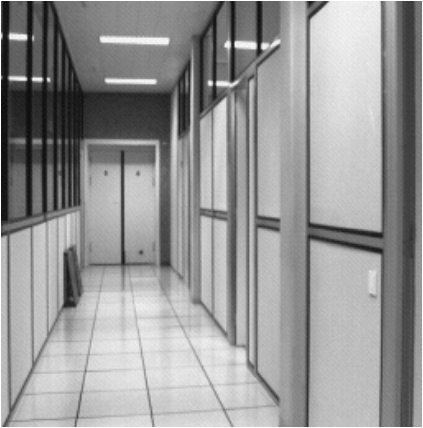
\includegraphics[width=0.25\textwidth]{resources/homograhpy_1.png} }}
                \qquad
                \subfloat[]{{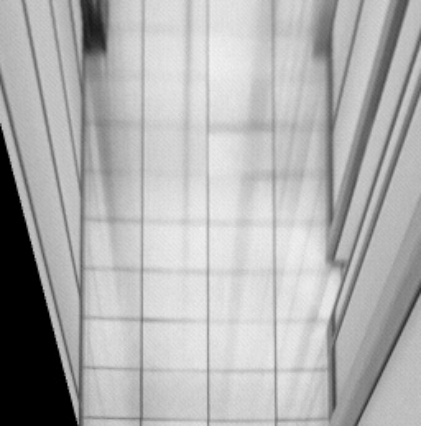
\includegraphics[width=0.25\textwidth]{resources/homography_2.png} }}
                \qquad
                \subfloat[]{{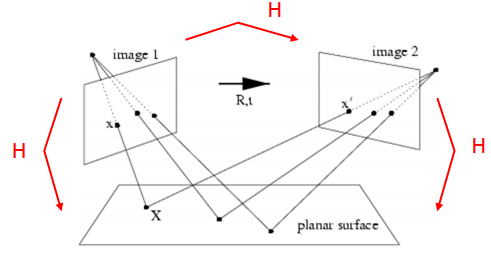
\includegraphics[width=0.35\textwidth]{resources/homography_3.png} }}
                \caption{Example of the 2-D projective transformation. a) Source image. b) Top-down view of the corridor floor generated from (a) using the four corners of a floor tile to compute the homography. c) A planar surface viewed by two camera positions is related by homography $H$, thus any point can be transformed between these different planes. Source: \cite{hartley2003multiple}}.
                \label{fig:homography_example}
            \end{figure}
  
        \subsection{Height estimation}
            In the previous section, we presented a 2-D transformation that can transform point coordinates between planes. This section deals with a related problem known as single-view metrology, which uses projective geometry to recover a structure of the 3-D world objects from a single image with several reference measurements. Since this section again contains complex theoretical concepts such as vanishing points, vanishing lines, we assume that the reader got acquainted with them from the suggested book \cite{hartley2003multiple}.
            
            Let us have a visible ground plane $p$ represented as a floor in the scene, the vanishing point $v$ in the vertical direction of the $p$, vanishing line $l$ of the $p$, $t_r$ and $b_r$ are the top and base points of the reference object, respectively and $t_x$ and $b_x$ are the top and base points of the object to be measured. All base points must lie on the $p$, and all top points must lie on a line that intersects the according to the base point and is perpendicular to $p$. Then, the $\alpha$ metric factor can be found by the following equation:
            \begin{equation}\label{height_equation_1}
                \alpha = - \frac{|| b_r \times t_r ||}{Z_r (l \cdot b_r) || v \times  t_r|| }.
            \end{equation}
            With the $\alpha$ calculated, we can estimate a height $Z_x$ for an arbitrary object that stands on the ground plane by the following equation:
            \begin{equation}\label{height_equation_2}
                  Z_x = - \frac{|| b_x \times t_x ||}{\alpha (l \cdot b_x) || v \times  t_x|| }.
            \end{equation}
            The application of this formula is most easily understood from Fig. \ref{fig:height_estimation} and the proof can be found in \cite{criminisi2002single}.
            
            To conclude, with this single-view metrology framework, we can measure the real-world height of the object that stands on the ground plane (with known $t_x$ and $b_x$ that are bounding box top or bottom point, respectively). It works for uncalibrated cameras, only real-world measurements on the ground plane and beyond are sufficient for calculating the $v$ and $l$. 

             \begin{figure}[h]
                \centering
                \subfloat[]{{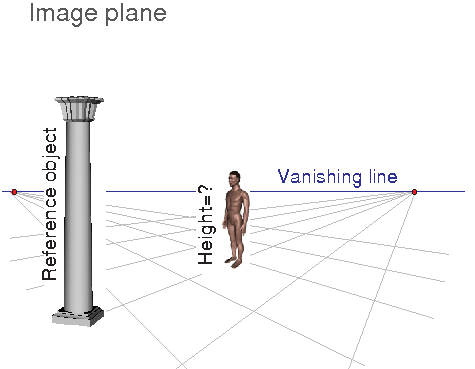
\includegraphics[width=0.4\textwidth]{resources/height_estimation_1.png} }}
                \qquad
                \subfloat[]{{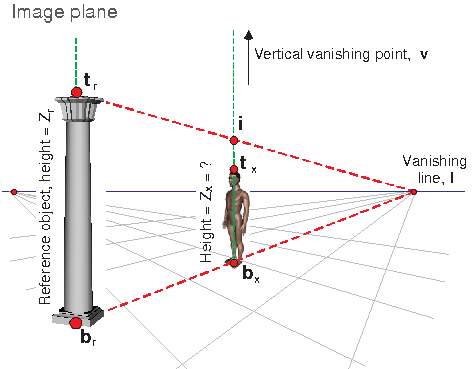
\includegraphics[width=0.4\textwidth]{resources/height_estimation_2.png} }}
                \qquad
                \subfloat[]{{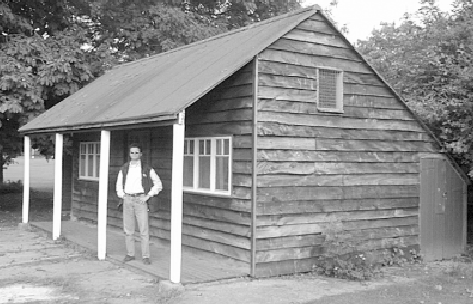
\includegraphics[width=0.4\textwidth]{resources/height_estimation_3.png} }}
                \qquad
                \subfloat[]{{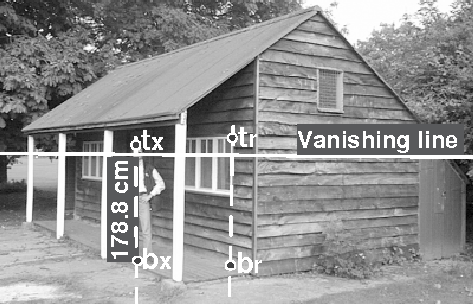
\includegraphics[width=0.4\textwidth]{resources/height_estimation_4.png} }}
                \caption{Measuring heights in single images. (a) The aim is to compute the height of the human figure relative to the height of the column (reference). The vanishing line of the ground plane has been computed and is shown blue. (b) The unknown height $Z_x$ can be computed from image quantities only as shown in \ref{height_equation_2} (c) A photograph of a garden shed in Oxford. (d) Once the height of the window top edge from the floor has been measured (reference), the height of the man is computed to be 178.8 cm which is about 1 cm off the ground truth. Source: \cite{criminisi2002single}}.
                \label{fig:height_estimation}
            \end{figure}
    \chapter{Implementation}
    This chapter contains information related to the implementation of the proposed framework. The whole implementation is done in Python language with the dependence on several other frameworks and libraries, including OpenCV, Tensorflow, and Darknet. The main application functionality spans eight Python modules.
    
\section{Module tracking\textunderscore app}
    This module is the main entry point of the application. It contains only one essential function that is responsible for running the proposed framework. In this function, we first load the input image stream, calibration parameters and other components such as object detectors, feature extractors, tracker, and image viewer. Then there is a loop that runs the algorithms as long as input frames are available. The application can be run either from an IDE or from the command line with various input parameters.

\section{Module detection}
    The detection module contains multiple wrappers for various object and face detectors proposed in \ref{detection_and_tracking_components}. It is responsible for loading these models based on input parameters, detecting objects in the input frame, and filtering detections by input criteria. 

\section{Module feature\textunderscore extraction}
    In this module, we propose to interface and pre-processing to various appearance feature extractors including age, gender, and emotion models, but also height estimator. The module also contains a function that assigns face regions to people bounding boxes.

\section{Module kalman\textunderscore filter}
    This module is vital for the proposed motion analysis method because it contains the configuration of the utilized filter. Our approach uses Kalman Filter implementation from famous FilterPy \cite{labbe2015kalman} library. The module is also responsible for converting filter's internal state to visualizable bounding box and for converting measurements to filter's input.

\section{Module matching}
    The matching module contains an efficient implementation of a proposed distance metric, namely the cosine metric for appearance (section \ref{appearance_metric}) and enhanced Euclidean distance for the state (section \ref{state_metric}). Metrics are calculated by NumPy, which is a high-performance linear algebra library written in C language. To make the computations as efficient as possible, we utilize the NumPy broadcasting technique.

\section{Module tracking}
    In the tracking module, we propose PeopleTracker class that is responsible for the actual matching of detections and tracks. It is mostly inspired by code from \cite{wojke2017simple}, but some modifications in the matching algorithm were made. Successfully matched tracks are updated from here, and unmatched detections are transformed to tentative tracks.
    
\section{Module track}
    An instance of Person class from the track module represents a single person that was detected in the scene. Each person instance has set of attributes including id, color for visualization, status, creation frame number, time since the last update, age in frame units, last body bounding box, last face bounding box, Kalman filter instance, and dictionary with gathered features.
    
\section{Module output\textunderscore statistics}
    This module is responsible for transforming all possible data to brief output statistics. It includes a class TrackingEvaluator which evaluates the tracking performance of the algorithm based on provided annotations. Class OutputStatistics is responsible for converting gathered data about people to usable outputs.

\section{Module visualization}
    Visualization module contains all drawing related functions including plotting output graphs using Matplotlib and Seaborn libraries. It implements an ImageViewer class that is responsible for showing the preview of processed images. The ImageViewer class also contains functionality that allows easier debugging by allowing users to pause the algorithm or process the stream by one frame at a time.
    \chapter{Evaluation}
In this chapter, we firstly discuss the reason behind creating a new dataset. We further present achieved results with our proposed framework, and lastly, we propose additional improvements for future work.

\section{Dataset}
    There are many public annotated datasets \cite{MOTChallenge2015, ferryman2009pets2009, zhuvisdrone2018} for a person tracking task and many others targeting soft-biometrics \cite{goodfellow2013challenges, yang2016wider}. However, their focus is a little different than what is needed for the evaluation of this thesis. Firstly, individuals only appear in a few images of the sequence, which is not entirely the case for retail, where it is required to maintain the individual's long-term identity even in the case of multiple occlusions. Secondly, these datasets do not focus on the joint task of tracking and soft-biometrics extraction. The available tracking sequence lacks additional information about people and the scene parameters that are required to calibrate the camera. It was, therefore, advisable to create an in-the-wild dataset to simulate a real scenario.
    
    The 14th floor of the \gls{fce} \gls{ctu} building was used to create a dataset, where it was possible to place a camera to a place that is most similar to the retail case. In total, over 10,000 images were captured, of which 2463 frames were hand-annotated with person bounding-boxes and identities. There are a total of 7028 bounding boxes with 11 person identities. Face regions were not annotated because it would have no added value for the evaluation. Related individual's soft-biometrics data such as age, gender, and height are known, but ground-truth data for emotions and trajectories are not available. There are only male representatives in the dataset. Captured frames are not further pre-processed.
  
\section{Hardware and software setup}\label{evaluation_estup}
    The speed performance of algorithms is tightly dependent on the utilized hardware and software setup. The proposed methods were tested on the computer available in \gls{improlab}. The testing setup consisted of Intel~i5~-~7600K~@~3.80GHz, NVIDIA GeForce RTX 2080 TI, 16 GB RAM, and SSD disk. The software dependencies were CUDA 10, cuDNN 7.5, Tensorflow 1.13, OpenCV 3.4.2, and the latest version of Darknet. All third-party libraries were compiled for GPU support.

\section{Tracking results}
    In order to be able to compare individual tracking solutions among each other, it is necessary to determine a suitable metric. Because metrics for object detection and tracking in the video can often be non-intuitive and complex, the well-known \gls{motp} and \gls{mota} metrics are adopted in this work. \gls{motp} metrics focus on the quality of detected regions, while \gls{mota} focuses on tracking accuracy, and its calculation affects the number of \glsentryfull{fp}, \glsentryfull{fn}, and \glsentryfull{idsw}. Factors affecting \gls{mota} are also compared, as it is interesting to see how they change depending on the detection network. The metrics are described in more detail in section \ref{evaluation-metrics}; however, to be concise, higher \gls{mota} or \gls{motp} means better.
    
    We present our results in table \ref{table:tracking_results} for different object detection architectures -- \gls{yolo}v2, \gls{yolo}v3, \gls{yolo}v3 \gls{spp}, and \gls{faster r-cnn} with ResNet50 backbone. For the retail usage, the number of identity switches (\gls{idsw}) is a crucial metric, and in this aspect, the \gls{faster r-cnn} outperformed other detectors by a large margin. We also provide some output predictions in Fig. \ref{fig:examples_of_outputs} and example video in \cite{trackingvideo} demonstrating robustness of the proposed algorithms.  
    
    \begin{table}[h]
        \centering
        \begin{tabular}{|c|c|c|c|c|}
            \hline
            \rowcolor{Blue}
            \color{White}\textbf{} & \color{White}\textbf{\gls{yolo}v2} & \color{White}\textbf{\gls{yolo}v3} & \color{White}\textbf{\gls{yolo}v3 SPP} & \color{White}\textbf{\gls{faster r-cnn}} \\ \hline \hline
                \gls{motp} & 0.795 & 0.84 & 0.89 & 0.87 \\ \hline
                \gls{mota} & 0.825 & 0.94 & 0.905 & 0.94 \\ \hline
                \gls{fn} & 879 & 306 & 470 & 228 \\ \hline    
                \gls{fp} & 147 & 132 & 223 & 167 \\ \hline    
                \gls{idsw} & 14 & 8 & 10 & 2 \\ \hline
                \gls{fps}  & 26.62 & 22.2 & 16.29 & 17.37 \\ \hline    
        \end{tabular}
        \caption{Tracker evaluation table.}
        \label{table:tracking_results}
    \end{table}
    
    \begin{figure}[h]
        \centering
        \subfloat[]{{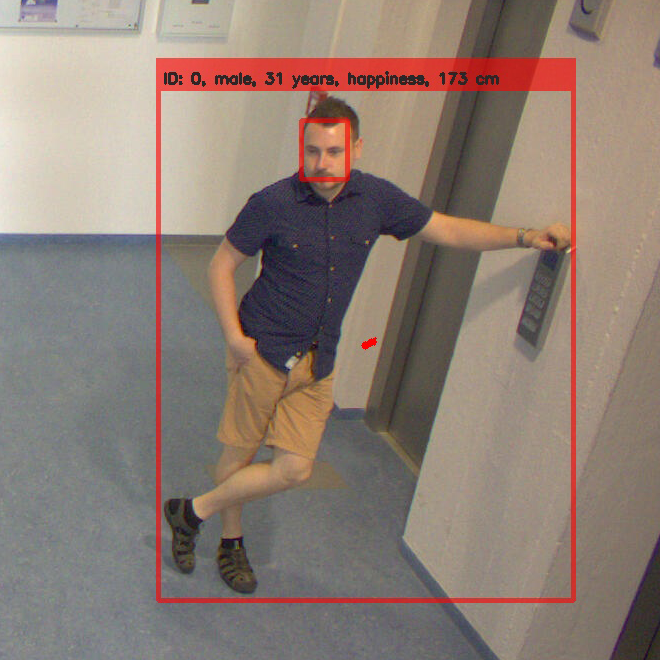
\includegraphics[width=0.28\textwidth]{resources/framework_example_1.png} }}
        \qquad
        \subfloat[]{{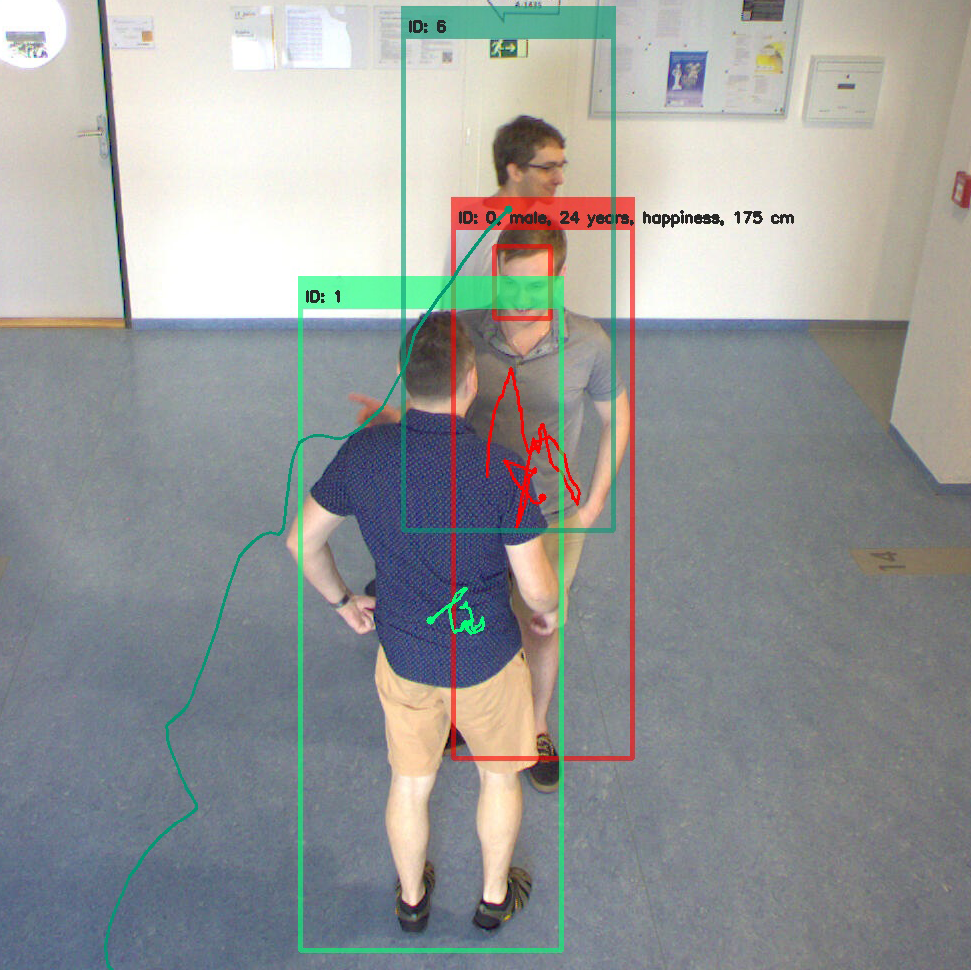
\includegraphics[width=0.28\textwidth]{resources/framework_example_2.png} }}
        \qquad
        \subfloat[]{{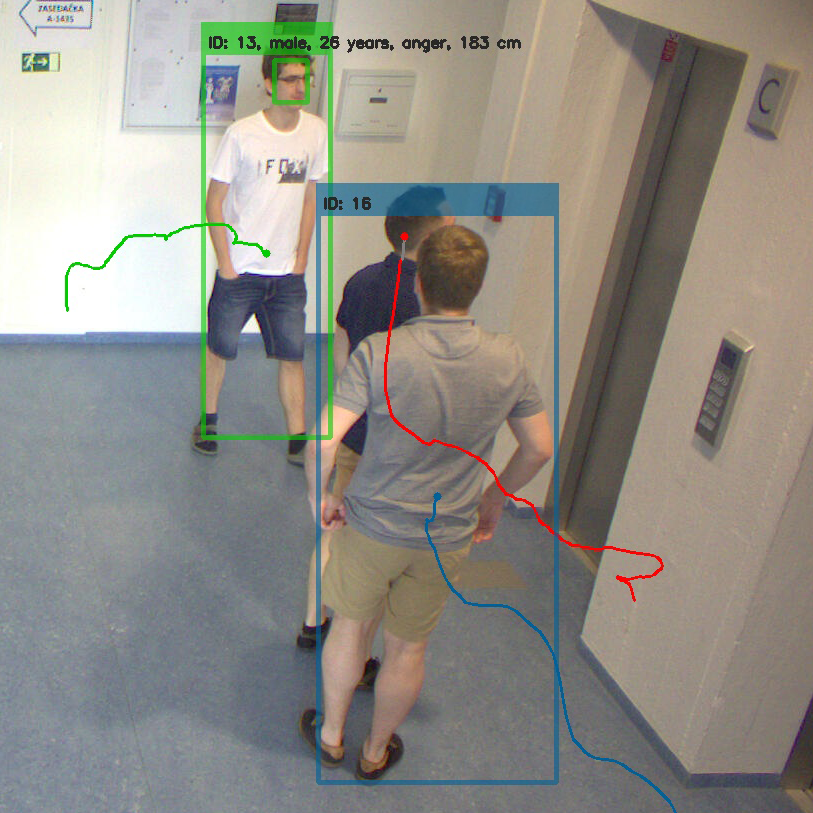
\includegraphics[width=0.28\textwidth]{resources/framework_example_3.png} }}
        \caption{Image examples of our framework. (a) An example of a person facing the camera so his biometrics can be accurately estimated. Only the height value is inaccurate by 2 cm, which is a very precise outcome. (b) An example of people who are close to each other without affecting the tracker accuracy. (c) An example of people who are even closer than in (b). The person in the middle is fully occluded, and no detection is available for him. However, the red circle is trying to predict his position, in case he reappears in the scene. The prediction of soft-biometrics for the person with ID 13 is inaccurate by one year and 3 cm.}
        \label{fig:examples_of_outputs}
    \end{figure}

    In the table with results, we can see that the more complex the architecture employed, the more accurate the results, which again verified the fact presented in the introduction chapter, that a robust object detector is a key to proper tracking. Specifically, we can observe the number of missed detections (\gls{fn}) and identity switches (\gls{idsw}) is decreasing with more robust architecture. \Gls{faster r-cnn} generally has more "ghost" detections (\gls{fp}), but it was something we expected already in the Methodology chapter, and it is not such a problem that would significantly affect the results of the framework. 
    
    Interesting observations are worse results achieved by the modified \gls{yolo}v3 with \glsentryfull{spp} architecture. According to the original paper, it should work better on small objects, and although it provided more accurate bounding boxes (\gls{motp}), all other aspects suggest that it is not very suitable for tracking algorithms.  
    
    The fact that FPS is decreasing with the complexity of object detector architecture is no surprise. Generally speaking, the bottle-neck of the tracker is the object detector. Based on our observations and measurements, the tracking algorithm without the object detector component can run at around 500 \gls{fps}. It is, therefore, necessary for any task to select the suitable object detector first. In our case, even with the complex \gls{faster r-cnn}, the tracking achieves near real-time performance.
    
\section{Soft-biometrics results}
    The evaluation of soft-biometrics is a bit more complicated. It is not possible to obtain precise ground-truth for trajectories and emotions, so there is no room for evaluation. However, three more remaining features could be possibly evaluated -- age, gender, and height. We decided to choose only age and height for the evaluation because we could not find a female representative at the time of the dataset creation. 
    
    The situation is even more complicated because some biometric information cannot always be extracted. It may happen that a person will always be back to the camera and it will not be possible to extract his facial information, or a person moves very fast or is occluded all the time, so it is not possible to estimate his height. Therefore, we only evaluate cases where it is possible to extract suitable soft-biometric data.
    
    We use \glsentryfull{mae} metric described in section \ref{evaluation-metrics} for evaluation instead of \gls{rmse} because it has easier interpretation. Description of the utilized detectors can be found in Methodology chapter. 
    
    In table \ref{table:age_estimation_results}, we present our outcome for age estimation for various face detectors. From the results, we can observe that the alignment feature in MTCNN has a great positive impact on accuracy, but it drastically reduces the \gls{fps}. Tensorflow Mobilenet \gls{ssd} architecture provides the best trade-off between performance (\gls{fps}) and accuracy (Age \gls{mae}).

    \begin{table}[h]
        \centering
        \begin{tabular}{|c|c|c|c|}
            \hline
            \rowcolor{Blue}
            \color{White}\textbf{} & \color{White}\textbf{faced} & \color{White}\textbf{Mobilenet \gls{ssd}} & \color{White}\textbf{MTCNN} \\ \hline \hline
                Age \gls{mae} & 5.21 & 3.82 & 2.65  \\ \hline
                \gls{fps} & 78.41 & 119.86 & 7.01 \\ \hline
        \end{tabular}
        \caption{Age estimation evaluation table.}
        \label{table:age_estimation_results}
    \end{table}

    The last table \ref{table:height_estimation_results} focuses on the influence of object detector on height estimation. \Gls{yolo} architectures generally provide less accurate bounding boxes, thus making the height error larger. The achieved results correspond to the \gls{motp} outcome in table \ref{table:tracking_results}. We can also see that the speed performance degradation compared to the original \gls{fps} is negligible. To conclude, height estimation works well in most cases, and it has a little computational overhead.
    
       \begin{table}[h]
        \centering
        \begin{tabular}{|c|c|c|c|}
            \hline
            \rowcolor{Blue}
            \color{White}\textbf{} & \color{White}\textbf{\gls{yolo}v2} & \color{White}\textbf{\gls{yolo}v3} & \color{White}\textbf{\gls{faster r-cnn}} \\ \hline \hline
                Height \gls{mae} & 7.31  & 5.84 & 4.09  \\ \hline
                \gls{fps} & 26.35  & 21.97 &  17.17 \\ \hline
        \end{tabular}
        \caption{Height estimation evaluation table.}
        \label{table:height_estimation_results}
    \end{table}
    
\section{Further work}
    This complicated and broad task is not something that can be fully accomplished in one final thesis. Therefore, in this section, we suggest some improvements for future work.
    
    \subsection{Tracking improvements}
        Current state-of-the-art object detectors are already achieving outstanding results. People are detected in most cases when they are visible. The problem arises when people are entirely occluded, so they are not visible to the camera, but we still need to retain their identity when they show up. This is a situation where having robust tracker helps. 
        
        Our tracker can deal with short-term occlusions which are mostly situation when people pass by. However, it is not designed for the case when individuals are completely missing for a few seconds. To improve in this manner, the missing tracks would need to be kept in the memory for a more extended period than 50 frames, but also a new matching metric for these cases would need to be developed.
        
        The tracking performance could also be improved by adding a non-linear state filter such as unscented Kalman filter or particle filter, which would improve the matching phase. The reason is that not all people behave linearly in their movement. Therefore, the current filter may occasionally diverge.

        From our observation, utilized object detectors are already robust with default parameters and pre-trained models. Therefore, there is no reason for re-training them for a particular task with people. There could be significant speed-up improvement by proposing an object detector that can detect faces and people simultaneously.

    \subsection{Soft-biometrics extraction improvements}
        Our framework can extract face information (age, gender, emotion), height, and trajectory. This information can only be obtained under certain conditions. If no face is visible during the whole tracking session, then it is not possible to output any face information. If the object moves quickly, then extracted height information is not accurate. Moreover, if an object is occluded, then trajectory information might contain gaps.
        
        Of course, all these shortcomings could be improved, but the significant improvement, for now, would be retraining the face extraction models on more in-the-wild data to improve the accuracy. There is no need to replace utilized architectures as they achieve state-of-the-art performance on current datasets, but it is needed to fine-tune the weights by faces that are captured at an angle, not only from the front view. It would also help to evaluate the methods on data from multiple environments and with more types of people.
        
        Another improvement could be achieved by employing a model that can do face embedding. This embedding then could be used in the matching phase to recover long term occluded individuals. 
    \begin{conclusion}
    This work was focused on building a framework for the task of people tracking and soft-biometric data extraction. In the introductory chapter, we thoroughly described the assignment with sufficient motivation, but also with its challenges. In the following theoretical chapter, we have described the necessary theoretical background in detail for understanding of this thesis. In chapter \ref{related_work}, we briefly reviewed the existing solutions, and based on that some popular methods were implemented from scratch or customized from open-source repositories to meet the thesis goals. The implemented solution is then evaluated in the evaluation chapter, and further improvements are proposed. The result is a functioning people tracking and soft-biometrics extracting framework that can be deployed in a real-world application.
    
    According to the table \ref{table:tracking_results}, the proposed algorithms achieve {state-of-the-art} results in long-term people tracking. The best solution based on \gls{faster r-cnn} achieves only two identity switches on our dataset, which is an outstanding outcome. The quality of the detected boxes is also very high. Evaluated height and age estimators achieve exact results. However, in future work, it is necessary to evaluate more individuals.
    
    The proposed methods are designed in several variations to meet different trade-offs of accuracy versus computational expensiveness, and since the final design of the framework is fully modular, it can be easily configured to meet demands for various other scenarios. We put much effort into the application design as a whole so that it can be easily expanded and it can now be deployed in real-world applications. There are still some shortcomings in the framework, but they are described so that they can be further worked on and we hope that this work will be a useful as a starting point for other people interested in this topic. 

\end{conclusion}
    
    % bibliography
    \bibliographystyle{prefs/iso690}
    \bibliography{ref}
    
    \appendix
    
    % acronyms
    \printglossaries
    
    % media contents
    \chapter{Media contents}\label{app:CDcontent}
    \begin{figure}
    	\dirtree{%
    		.1 readme.txt\DTcomment{the file with CD contents description}.
    		.1 data\DTcomment{the data files directory}.
    		.2 example\textunderscore sequence\DTcomment{the directory with example sequence from dataset}.
    		.3 *.jpg\DTcomment{the example images}.
    		.2 example\textunderscore sequence\textunderscore graphs\DTcomment{the directory of graphs of experiments}.
    		.3 *.png\DTcomment{the motion output graphs}.
    		.2 tracking\textunderscore example.mp4\DTcomment{the example video file}.
    		.1 src\DTcomment{the directory of source codes}.
    		.2 models\DTcomment{the directory of deep learning modules}.
    		.2 utils\DTcomment{the directory of helper modules}.
    		.2 *.py\DTcomment{the Python source files}.
    		.1 text\DTcomment{the thesis text directory}.
    		.2 thesis\DTcomment{the directory of \LaTeX{} source codes of the thesis}.
    		.2 thesis.pdf\DTcomment{the Diploma thesis in PDF format}.
    	}
    \end{figure}
    

\end{document}
